% Chapter Template

\chapter{The flip flop qubit} % Main chapter title

\label{Chapter2} % 

\HRule
\vspace{0.5cm} \hspace{2cm}
\small
\hangindent=4cm
\\
        ``\emph{Scalability is the future}"
\\ \\
\hangindent=4cm
\begin{flushright}
--? \\
\end{flushright}

\vspace{0.5cm}

\noindent \HRule
\clearpage

As discussed in chapter \ref{sec:scaleup}, new ideas for long range, scalable coupling are necessary to advance silicon quantum computing. This chapter presents a new type of qubit that relies on electric dipole interactions and aims to answer this demand. 

\section{A new electrically accessible qubit}

\begin{figure}[h]
	\centering
	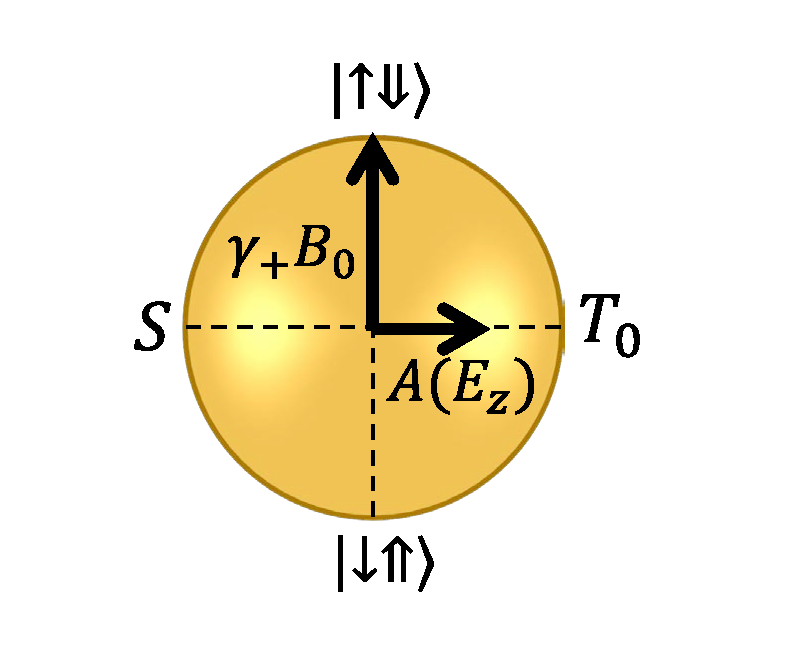
\includegraphics[width=0.5\columnwidth]{polished/ff_blochsphere.pdf}
	\caption[Flip-flop qubit Bloch sphere]{\textbf{Flip-flop qubit Bloch sphere.} Bloch sphere of a flip-flop spin qubit in an external magnetic field $B_0$ coupled to a vertical electric field $E_z$ via the hyperfine interaction $A$. Electron-nuclear singlet and triplet states are denoted by $S=\left(\ket{\downarrow\Uparrow}-\ket{\uparrow\Downarrow}\right)/\sqrt{2}$ and $T_0=\left(\ket{\downarrow\Uparrow}+\ket{\uparrow\Downarrow}\right)/\sqrt{2}$.}
	\label{fig:ff_blochsphere}
\end{figure}

\cite
The new qubit is based on the phosphorus donor qubit as described in section \ref{sec:donorqubit}. However, instead of encoding the quantum information in just the electron or the nuclear spin, we define a new qubit with the anti-aligned spin states $\ket{\downarrow\Uparrow}, \ket{\uparrow\Downarrow}$ as the basis. We call this the flip-flop qubit. This transition is not magnetically accessible as the total z-angular momentum is constant. However, the hyperfine interaction $H=A\bm{S\cdot I}$ is a transverse term for this states with its eigenstates $S=\left(\ket{\downarrow\Uparrow}-\ket{\uparrow\Downarrow}\right)/\sqrt{2}$ and $T=\left(\ket{\downarrow\Uparrow}+\ket{\uparrow\Downarrow}\right)/\sqrt{2}$ (see figure \ref{fig:ff_blochsphere}) and thus can be used to drive the transition. 
The flip-flop qubit energy splitting is 
\begin{equation} \label{eq:e_ff}
\epsilon_{\rm ff}(A)=\sqrt{\left(\gamma_+B_0\right)^2+A^2},
\end{equation}
where $\gamma_+=\gamma_e+\gamma_n$. Is $A$ now modulated at frequency $\epsilon_{ff}$, we are driving the flip-flop transition with electric dipole spin resonance (EDSR). 

The hyperfine interaction strength between the electron and the nucleus depends on the overlap of the electron wave function with the nucleus position $A\sim |\psi(0,0,z_d)|^2$. Hence, by reducing said overlap, the interaction can be decreased. This can be achieved by applying an electric field on top of donor that pulls the electron from the donor to the SiO2 interface, where it behaves like a quantum dot. The electron position is described by the orbital degree of freedom

\subsection{Manipulating the orbital degree of freedom: the charge qubit} \label{sec:chargequbit}

When the electron is at the donor, the ground orbital wavefunction $\ket{d}$ is a symmetric combination of the 6 valleys $\mathrm{k_{\pm x}}$, $\mathrm{k_{\pm y}} $, $\mathrm{k_{\pm z}} $ (see chapter \ref{sec:silicon}). The next valley-orbit states are $11.7\,$meV higher in energy and thus can be neglected. When the electron is confined at the interface, in a quantum dot like state, in-plane strain splits off the in-plane $k_{\pm x}, k_{\pm y}$ valleys so that the wave function lives in the z valleys $k_{\pm z}$ where the remaining twofold degeneracy is lifted by the electronic z confinement into a lower valley $\ket{i}$ and a higher valley $\ket{v}$. The remainder of the excited donor and dot states are well above the ground states by several meV \cite{Rahman2009, Calderon2009}. Thus, close to the ionization point, the lowest-energy sates of the system are $\ket{d}, \ket{i}, \ket{v}$ as shown in figure \ref{fig:nemolevels} inset. 
These levels can by computed with atomistic tight binding calculations using the package NEMO-3D \cite{Klimeck2007a, Klimeck2007b} with donor depth $z_d=15.2\,$nm below the Si/SiO2 interface and the donor biased close to ionization $E_z^0$. Figure \ref{fig:nemolevels} shows the dependence of the energy levels on the electric field $E_z$ with the dots indicating the tight binding simulations. 

\begin{figure}[h]
	\centering
	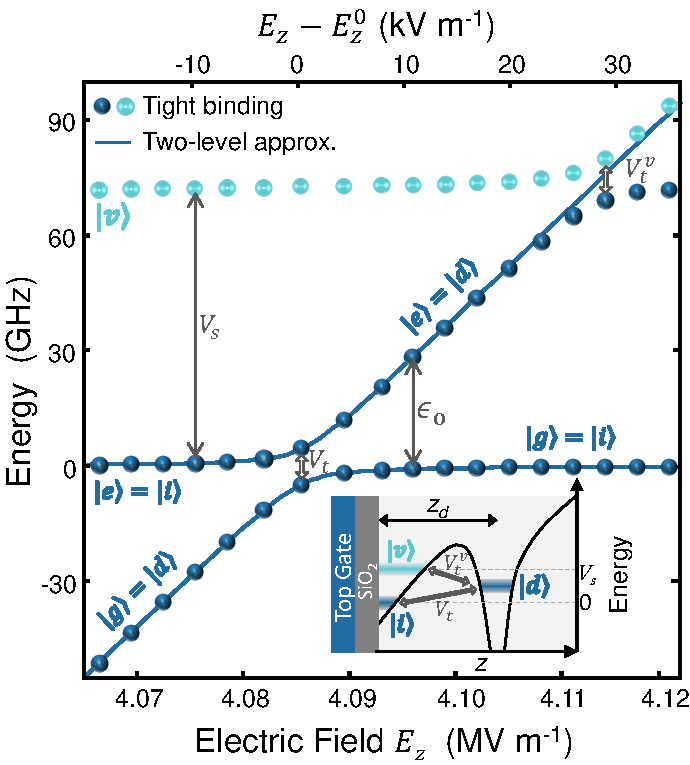
\includegraphics[width=0.7\columnwidth]{Nemolevels}
	\caption[Orbital and valley states]{\textbf{Orbital and valley states.} The lowest orbital energy levels of the donor-interface system, with respect to the lower valley interface state $\lvert i \rangle$ (set as the zero-energy reference). The donor is assumed 15.2 nm below a Si/SiO$_2$ interface. The dots correspond to the energy levels obtained from a full-scale tight-binding calculation with NEMO-3D. Solid lines represent the energy levels obtained from the two level approximation described by Eq. \ref{eq:H_orb}. Inset: Potential profile as a function of depth, illustrating the donor $\lvert d \rangle$, lower $\lvert i \rangle$ and upper $\lvert v \rangle$ valley interface states. The donor ground state is tunnel-coupled to the lower and upper valley interface states by $V_t$ and $V_t^v$  respectively.}
	\label{fig:nemolevels}
\end{figure}

We find that the electron orbital charge qubit degree of freedom can be approximated by a two-level system with ground state $\ket{g}$ and excited state $\ket{e}$ for $E_z<E_z^v\sim 4.11\,$MV/m when the third valley state $\ket{v}$ becomes relevant. 

When $E_z \ll E_z^0$, the charge qubit ground state $\lvert g \rangle $ consists of the electron being  localized at the donor, $\ket{d}$, whereas the first excited state $\lvert e \rangle $ corresponds to the lower valley interface state $\ket{i}$. 
With increasing $E_z$, the two states approach, and anticross at the ionization point $E_z = E_z^0$ and $\ket{d}$ is the excited state for $E_z \gg E_z^0$, until it eventually anticrosses with the upper valley interface state$\ket{v}$ at $E_z^v$. 

We can describe this charge qubit with the Pauli matrices 
\begin{equation}\sigma_x=\begin{pmatrix}0 & 1\\1 &0 \end{pmatrix}, \sigma_y=\begin{pmatrix}0 &-i\\i &0 \end{pmatrix}, \sigma_z=\begin{pmatrix}1 &0\\0 &-1 \end{pmatrix}.
\end{equation} 
Choosing $\ket{d}=\begin{pmatrix}0\\1 \end{pmatrix},\ket{i}=\begin{pmatrix}1\\0\end{pmatrix}$ as the basis states the corresponding Hamiltonian is
\begin{equation} \label{eq:H_orb}
\mathcal{H}_{\rm orb}=\frac{V_t \sigma_x-\left[e(E_z - E_z^0) d/h\right]\sigma_z}{2},
\end{equation}
(solid lines in figure \ref{fig:nemolevels}) with an energy separation between the two levels of 

\begin{equation} \label{eq:e_o}
\epsilon_{\rm o}=\sqrt{\left(V_t\right)^2+\left[e(E_z - E_z^0) d/h\right]^2}.
\end{equation}

where $V_t=9.3\,$GHz is the tunnel coupling between the donor and the interface potential wells (at $z_d=15.2\,$nm), $E_z^0$ is the vertical electric field at the ionization point and $h$ is the Planck constant. The charge qubit energy is plotted in figure \ref{fig:chargequbit}.  We find that $d=11\,$nm which represents the separation between the center-of-mass positions of the donor $\ket{d}$ and interface $\ket{i}$ orbitals and is expectedly lower than the donor depth $z_d$.

\begin{figure}[h]
	\centering
	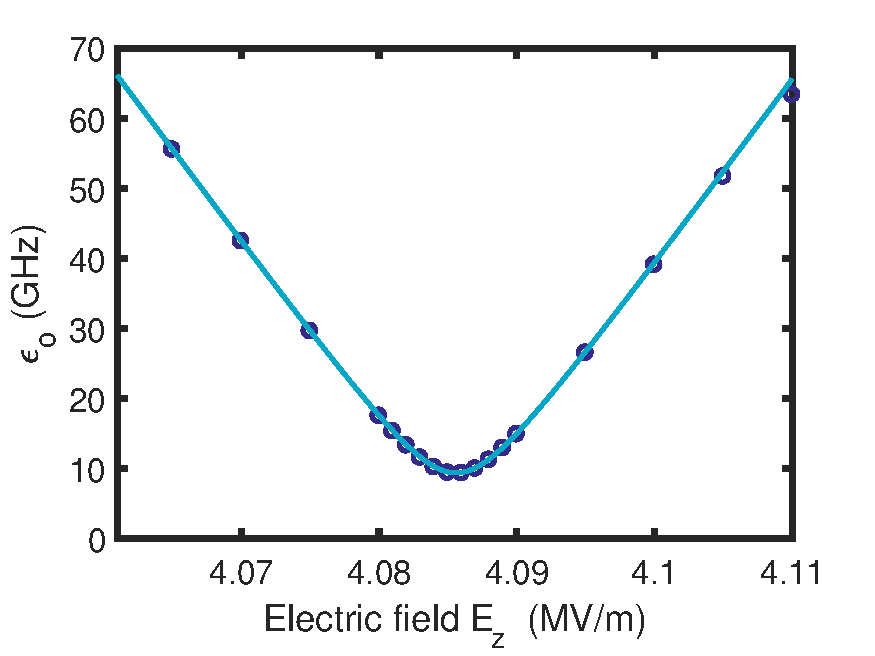
\includegraphics[width=0.8\columnwidth]{polished/chargequbit_dispersion.pdf}
	\caption[Charge qubit dispersion relation]{\textbf{Charge qubit dispersion relation.} Charge qubit dispersion relation $\epsilon_0$ as a function of vertical electric field $E_z$, for $V_t=9.3\,$GHz, $d=11nm$ and $E_z^0=0\,$V. The dots are obtained by NEMO-3D full-scale tight binding simulation while the line corresponds to the two-level approximation, giving eq. \eqref{eq:e_o}.}
	\label{fig:chargequbit}
\end{figure}

At the ionization point $E_z^0$ the basis states of the charge qubit are $\ket{g}=\frac{\ket{i}-\ket{d}}{\sqrt{2}}=\frac{1}{\sqrt{2}}\begin{pmatrix}-1\\1\end{pmatrix}$ and $\ket{e}=\frac{\ket{i}+\ket{d}}{\sqrt{2}}=\frac{1}{\sqrt{2}}\begin{pmatrix}1\\1\end{pmatrix}$ and $\epsilon_0=V_t$. 
If we were to express the charge qubit in this basis, we transform $\sigma_z\leftrightarrow-\sigma_x$ in $H_{orb}$.

More generalized we can express the charge qubit eigenstates as
\begin{eqnarray}\label{eq:chargestates}
\ket{e}&=&\alpha_1 \ket{i}+\beta_1\ket{d}=\begin{pmatrix}\alpha_1\\ \beta_1\end{pmatrix}\\
\ket{g}&=&\alpha_2 \ket{i}+\beta_2 \ket{d} =\begin{pmatrix}\alpha_2\\ \beta_2\end{pmatrix}
\end{eqnarray} with $\alpha_{1,2},\beta_{1,2}$ depending on $V_t$ and $E_z$. 


\paragraph{Modulating the hyperfine interaction}
 

\begin{figure}[h]
	\centering
	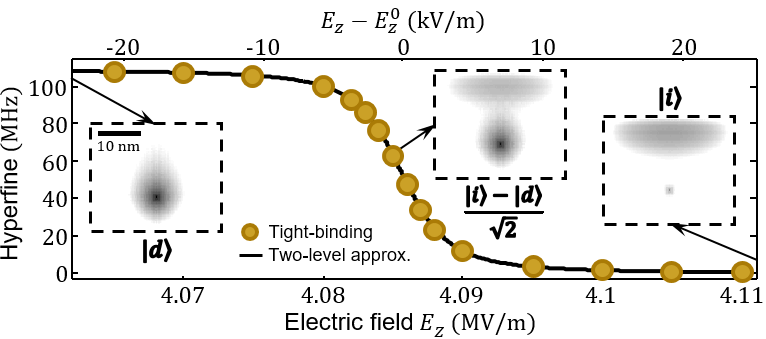
\includegraphics[width=0.9\columnwidth]{hfchange.png}
	\caption[Hyperfine interaction change with electric field]{\textbf{Hyperfine interaction change with electric field} Atomistic tight-binding simulations \cite{Klimeck2007} (dots) of the electron-nucleus hyperfine interaction, for a $z_d=15.2$~nm deep donor, as a function of vertical electric field. The solid line is a fit using the simplified two-level Hamiltonian $\mathcal{H}_{\rm orb}+\mathcal{H}_A^{\rm orb}$, which yields $V_t=9.3$~GHz (see \ref{App:Nemo-orb}). The insets show the electron ground-state wavefunction, $\ket{g}$ for three different vertical electric fields.}
	\label{fig:hfchange}
\end{figure}

As the hyperfine coupling the electron and nucleus experience depends on the wave function overlap between electron and nucleus, it depends on the state of the charge qubit. Is the charge qubit in the donor state $\ket{d}$, the hyperfine is full strength $A$ while the hyperfine is $0$ if it is in the interface state $\ket{i}$. Thus we can describe the orbital dependent hyperfine Hamiltonian as 

\begin{equation} \label{eq:H_A}
\mathcal{H}_{A}^{\rm orb}=A\left(\frac{1 - \sigma_z}{2}\right){\bf S\cdot I}
\end{equation}

Figure \ref{fig:hfchange} shows the hyperfine strength with applied electric field. The dots present the tight-binding simulations with NEMO-3D. The line is derived from the Hamiltonian by calculating the ground state eigenvector $\ket{g}$ and measuring its expectation value 

\begin{equation}\label{eq:AE}
A(E_{dc})=\langle g|A\left(\frac{1 - \sigma_z}{2}\right)|g\rangle=A|\beta_2|^2
\end{equation}. We find that both methods agree well which confirms our two-level approximation. The insets show the wavefunction at different electric fields. 

To determine the coupling between the charge qubit and the spin states $\ket{\downarrow\Uparrow}, \ket{\uparrow\Downarrow}$ we calculate the matrix transition element 
\begin{equation}\label{eq:g_so}
g_{so}=\langle g\uparrow\Downarrow|H_{A}^{orb}\ket{e\downarrow\Uparrow}=\frac{A}{4}\langle g|\sigma_z\ket{e} =\frac{A}{2}\left(\alpha_1\alpha_2^\dagger-\beta_1\beta_2^\dagger\right)
\end{equation}
At the ionization point $\langle g|\sigma_z\ket{e}=1$ and the coupling is the strongest, allowing for fast driving. To calculate $\langle g|\sigma_z\ket{e}$ outside the ionization point we need to determine $\alpha,\beta$ from equation \eqref{eq:chargestates} by calculating the eigenvectors $\ket{g},\ket{e}$. 

We generalize the problem to 

\begin{equation}
H=\begin{pmatrix}
-A & B\\
B & A
\end{pmatrix}
\end{equation}

The eigenvectors follow to

\begin{equation}
\begin{pmatrix}
-A-\lambda_{1,2} & B\\
B & A-\lambda_{1,2}
\end{pmatrix} \cdot 
\begin{pmatrix}
\alpha_{1,2} \\ \beta_{1,2}
\end{pmatrix} =
\begin{pmatrix}
0 \\ 0
\end{pmatrix}
\end{equation}

This gives the equations 
\begin{eqnarray}
\left(-A-\lambda_{1,2}\right)\alpha_{1,2}+B\beta_{1,2}=0 \label{eq:eigen1}\\
\alpha_{1,2}A+\left(A-\lambda_{1,2}\right)\beta_{1,2}=0
\end{eqnarray}
and the normalization condition
\begin{equation}\label{eq:norm}
\beta_{1,2}=\sqrt{1-\alpha_{1,2}^2}
\end{equation}
We insert equation \eqref{eq:norm} into \eqref{eq:eigen1} and get
\begin{eqnarray}
\alpha_{1,2}=\frac{1}{\sqrt{1+\frac{\left(A+\lambda_{1,2}\right)^2}{B^2}}}\\
\beta_{1,2}=\sqrt{1-\frac{1}{1+\frac{\left(A+\lambda_{1,2}\right)^2}{B^2}}}
\end{eqnarray}

with 
\begin{equation}
\lambda_{1,2}=\pm\sqrt{A^2+B^2}
\end{equation}
follows

\begin{eqnarray}\label{eq:ab}
\alpha_{1}=\frac{1}{\sqrt{\Phi^2+1}}=\beta_2=>\beta\\
\beta_{1}=\frac{\Phi}{\sqrt{1+\Phi^2}}=>\alpha\\
\alpha_{2}=\frac{1}{\sqrt{1+\Theta^2}}=-\beta_1=>-\alpha\\
\beta_{2}=\frac{\Theta}{\sqrt{1+\Theta^2}}=>\beta
\end{eqnarray}

where \begin{eqnarray}\label{eq:abcont}
\Phi=\frac{A+\sqrt{A^2+B^2}}{B}\\
\Theta=\frac{A-\sqrt{A^2+B^2}}{B}
\end{eqnarray}

This gives us the hybridized states 
\begin{eqnarray}\label{eq:hybridstates}
\ket{e}&=&\beta \ket{i}+\alpha\ket{d}\\
\ket{g}&=&-\alpha \ket{i}+\beta \ket{d}
\end{eqnarray}


Now we can calculate $A(E_{dc})$ with equation \eqref{eq:AE} to
\begin{equation}
A(E_{dc})=A\left(\frac{\Theta}{\sqrt{1+\Theta^2}}\right)^2=\frac{A}{2}\left(1-\frac{e\left(E_z-E_z^0\right)d/h}{\epsilon_0}\right)
\end{equation}
with $A=e\frac{\left(E_z-E_z^0\right)d}{2h}$ and $B=\frac{V_t}{2}$ 

and \eqref{eq:g_so} to
\begin{equation}
g_{so}=\frac{A}{4}\frac{V_t}{\epsilon_0}
\end{equation}

Here we have assumed that the hyperfine coupling between electron spin and $^{31}$P nucleus is purely isotropic \cite{Feher1959}, i.e. dominated by the Fermi contact hyperfine term. This assumption may no longer exactly hold when the donor electron wave function is distorted from its spherical symmetry in the presence of the strong vertical electric field, whereby a small dipolar component can be created (a related case, where the electron is shared between two proximal P donors, has been recently studied \cite{Hile2018}). However, it is known that the Fermi contact component of the hyperfine coupling for donor is silicon is always the dominant term, even for $^{29}$Si nuclei which are placed off-center with respect to the symmetry point of the wavefunction \cite{Ivey1975}. Therefore, we expect the isotropic approximation to capture the main physics of the problem.


\paragraph{The flip-flop qubit}

As we apply an external magnetic field $B_0$ to our system, we need to account for the Zeeman energy of both the electron and the nuclear spin. This energy depends on the gyromagnetic ratio. However, the electron gyromagnetic ratio $\gamma_e$ changes when the electron is confined at the Si/Sio2 interface, up to $0.7\%$ from the donor-bound electron \cite{Rahman2009}. We include this in the Zeeman Hamiltonian

\begin{equation} \label{eq:H_Zeeman_orb}
\mathcal{H}_{B_0}^{\rm orb}=\gamma_e B_0\left[1+\left(\frac{1+\sigma_z}{2}\right)\Delta_\gamma\right]S_z - \gamma_n B_0 I_z.
\end{equation}

Thus to describe the full physics of the flip-flop qubit we get

\begin{equation} \label{eq:H_ff_ge}
\mathcal{H}_{\rm ff} = \mathcal{H}_{B_0}^{\rm orb} +\mathcal{H}_{A}^{\rm orb} + \mathcal{H}_{\rm orb}.
\end{equation}

This system is composed of the three degrees of freedom, orbital, electron spin and nuclear spin which gives us a eight-dimensional Hamiltonian of
\begin{equation}
\mathcal{H}=H_{orb}\otimes H_{e}\otimes H_{n}
\end{equation}
with the unperturbed energy eigenstates $\{\ket{g}, \ket{e}\} \otimes \{\ket{\Uparrow}, \ket{\Downarrow}\} \otimes  \{\ket{\uparrow}, \ket{\downarrow}\}$ with the spin states pointing along the external magnetic field. 
As long as the Zeeman energy exceeds the hyperfine modulation characterized by $A/4$, the latter is a perturbation only and the energy eigenstates of $H$ remain the approximate products of the eigenstates. 
To calculate the flip-flop qubit energy we numerically determine the eigenvectors of $H_{ff}$ and find the ones with the largest overlap to the flip-flop states $\ket{g \Downarrow \uparrow}, \ket{g\Uparrow\downarrow}$ with the orbital state remaining unexcited. We then get the energy by calculating the difference of the corresponding eigenvalues. Thus we arrive at the curve plotted in yellow in figure \ref{fig:ff_energy}.

\begin{figure}[h]
	\centering
	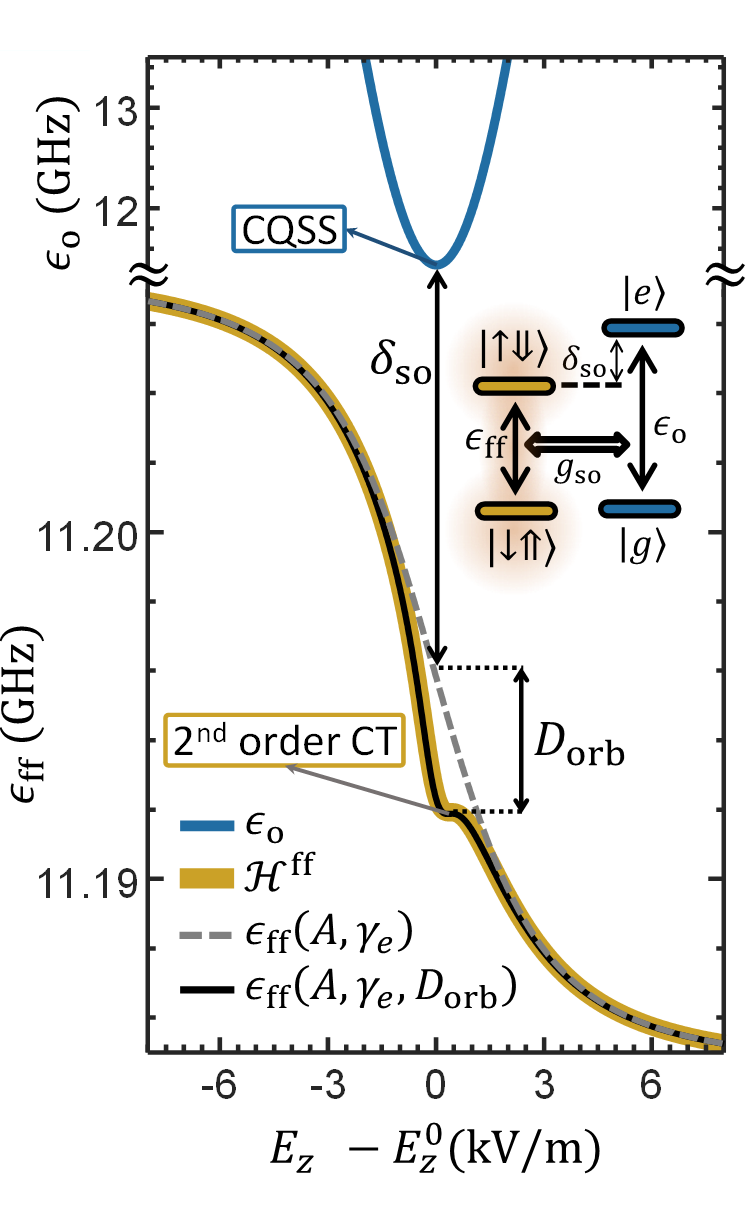
\includegraphics[width=0.6\columnwidth]{polished/ff_energy.png}
	\caption[Flip-flop qubit dispersion relation]{\textbf{Flip-flop qubit dispersion relation} Charge, $\epsilon_{\rm o}$, and flip-flop, $\epsilon_{\rm ff}$, qubits transition frequencies as a function of vertical electric field $E_z$, for $B_0=0.4$~T, $A=117$~MHz, $d=15$~nm, $\Delta_\gamma=-0.2\%$ and $V_t=11.44$~GHz. The inset shows the level diagram of flip-flop states coupled to charge states. CT stands for 'clock transition' and CQSS for 'charge qubit sweet spot'.}
	\label{fig:ff_energy}
\end{figure}

We can also determine the eigenvectors analytically. We have the ground state and two hybridized excited states
\begin{eqnarray}\label{eq:ff_hybrid}
\ket{\tilde{g}}=\ket{g\uparrow\Downarrow}\\
\ket{\tilde{e}_1}=\beta\ket{g\uparrow\Downarrow}+\alpha\ket{e\downarrow\Uparrow}\\
\ket{\tilde{e}_2}=-\alpha\ket{g\uparrow\Downarrow}+\beta\ket{e\downarrow\Uparrow}
\end{eqnarray}
where $\alpha$ and $\beta$ are determined by eq. \eqref{eq:ab} and \eqref{eq:abcont} with $A=\delta_{so}$ and $B=2g_{so}$.  Basically A describes the energy scale ($\sigma_z$) and B drives the transitions ($\sigma_x$). 

%When do i need to use these ones for g and e? whats with the g and e hybridization of i and d? 

When we compare this to formula \eqref{eq:e_ff} (plotted in dotted grey) we find a large deviation around the ionization point. There $\epsilon_{ff}(A,\gamma_e)$ shows a steep slope, mostly caused by the $E_z$-dependence of $\gamma_e$ as $\gamma_+B_0\gg A$ while $H_{ff}$ sees a dip. This dip is a result of the transverse coupling between the charge and spin states created by the hyperfine coupling in equation \ref{eq:H_A}. 

Figure \ref{fig:ff_energy} insert shows the energy levels for our qubit system. On the one hand, we have the charge qubit states $\ket{g}$ and $\ket{e}$ and on the other the spin flip-flop states $\ket{\downarrow\Uparrow}$ and $\ket{\uparrow\Downarrow}$ which are separated by $\epsilon_0$ and $\epsilon_{ff}$ respectively. Thus the charge and flip-flop qubit are detuned by $\delta_{\rm so}=\epsilon_{\rm o} - \epsilon_{\rm ff}$ but coupled with strength $g_{so}$. 

Due to the detuning the flip-flop transition is a second-order process. Furthermore, as $g_{so}\ll \delta_{so}$, the system is in the dispersive regime. This means that the flip-flop transition experiences an AC Stark shift which can be calculated with second order perturbation theory to

\begin{eqnarray} \label{eq:Dorb}
D_{\rm orb}(E_z)&=&\frac{\left| \langle \uparrow\Downarrow g|H_{orb}^A\ket{e\downarrow\Uparrow}\langle e\downarrow\Uparrow|H_{orb}^A\ket{g\uparrow\Downarrow}\right|}{E_{e\downarrow\Uparrow}-E_{g\uparrow\Downarrow}}\\
&=&\frac{[g_{\rm so}(E_z)]^2}{\delta_{\rm so}(E_z)},
\end{eqnarray}

\cite{Blais2004}, reducing the flip-flop qubit frequency to:

\begin{equation} \label{eq:e_ff_ge_Dorb}
\epsilon_{\rm ff}(A,\gamma_e,D_{\rm orb})=\epsilon_{\rm ff}(A,\gamma_e)-D_{\rm orb}(E_z).
\end{equation}

\begin{figure}[h]
	\centering
	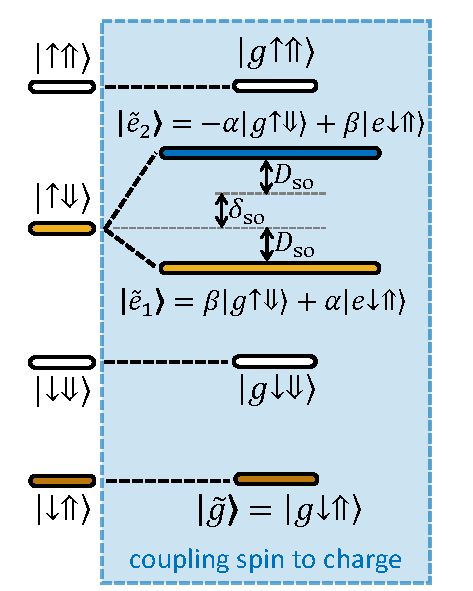
\includegraphics[width=0.5\columnwidth]{polished/hybridlevels.pdf}
	\caption[Hybridized charge-flip-flop states]{\textbf{Hybridized charge-flip-flop states} Level diagram showing the hybridization of the charge and flip-flop states due to the coupling $g_{so}$ when the detuning $\delta_{so}$ is small.}
	\label{fig:hybridlevels}
\end{figure}

Figure \ref{fig:hybridlevels} shows the full picture of the hybridized eigenstates with the AC stark shift for small detunings $\delta_{so}$. 

Around $E_z\approx E_z^0$ the charge qubit comes closet to the flip-flop qubit (see Fig. \ref{fig:clock}a) while the coupling $g_{\rm so}$ is highest. Consequently $D_{\rm orb}(E_z)$ is largest. Plotting Eq.~\eqref{eq:e_ff_ge_Dorb} (thin black line in Fig. \ref{fig:clock}a) agrees with the full numerical simulations of the Hamiltonian in Eq. \ref{eq:H_ff_ge}. 


\section{Electrical noise and relaxation} \label{sec:noise}

\paragraph{Dephasing due to electrical noise}

Since our qubit is based on the use of electric fields, the presence of electric noise is a concern for the longevity of our qubit states. Generally, to achieve a high qubit performance one needs a high ratio of qubit coherence time to qubit gate operation time. 

For the charge qubit we find that at the ionization point, the transition frequency exhibits a local minima equal to $V_t$ and is thus first order insensitive to electrical noise $\partial\epsilon_{\rm o}/\partial E_z=0$ (see figure \ref{fig:chargequbit}), called a clock transition. However, we do not intent to operate the charge qubit as its dephasing rate still exceeds $10^6\,$Hz. 

\begin{figure}[h]
	\centering
	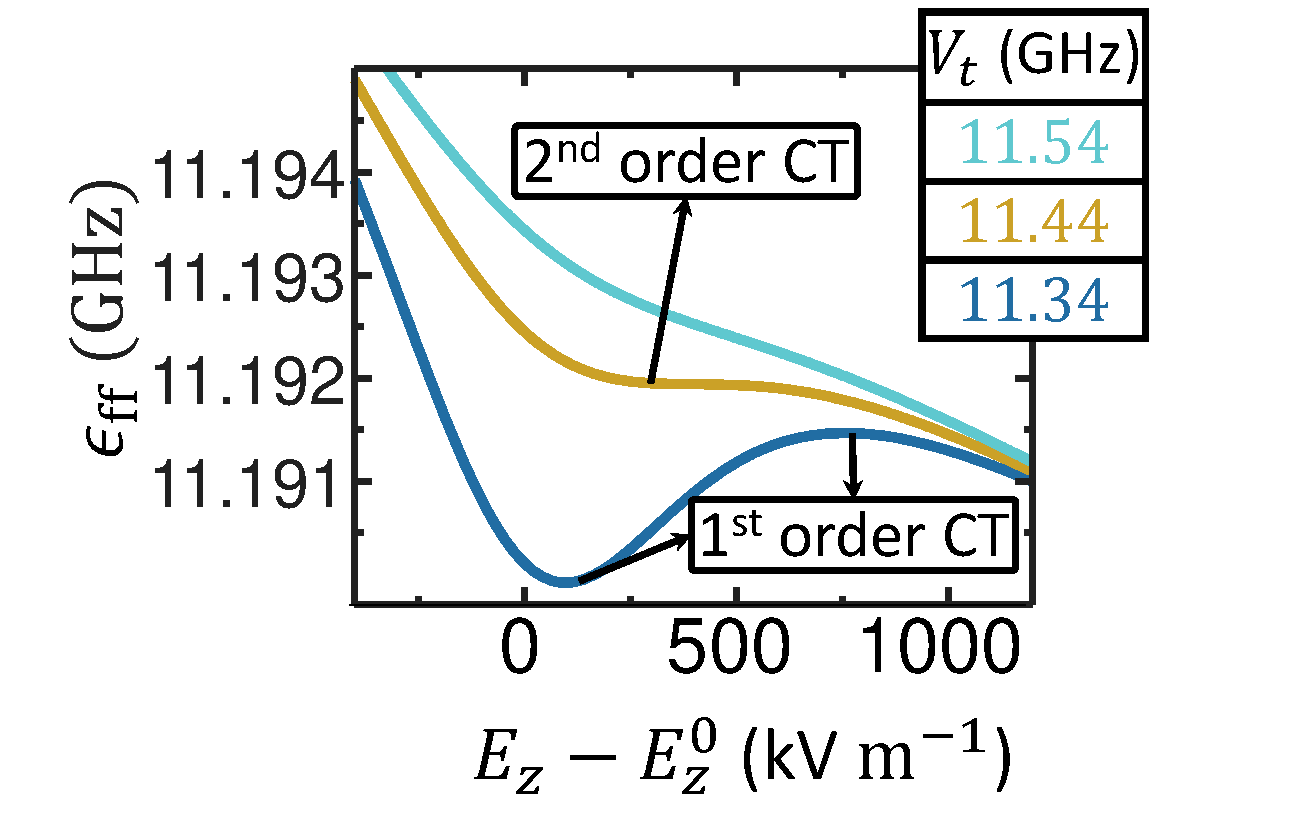
\includegraphics[width=0.75\columnwidth]{polished/ff_Vt.pdf}
	\caption[Flip-flop dispersion for different tunnel couplings]{\textbf{Flip-flop dispersion for different tunnel couplings} $E_z$-dependence of flip-flop precession frequency for the three indicated tunnel coupling values.}
	\label{fig:ff_Vt}
\end{figure}


Conveniently, the flip-flop qubit also exhibits a noise insensitive region close to the ionization point. The properties of this region depend on $V_t$. Figure \ref{fig:ff_Vt} shows 3 different values of $V_t$. For low $V_t$ the dispersive shift is strong due to the closeness of the charge qubit and thus creates two first order clock transitions. These merge into one for $V_t=11.44\,$GHz. This creates a second-order clock transition and strongly reduces dephasing. Finally, for high $V_t$ the dispersive shift is not strong enough and does not yield a minimum. 

We estimate the dephasing from quasi-static $E_z$ noise. This is noise with a spectral weight centred at frequencies smaller than the qubit resonance and Rabi frequency, aligned with the donor-dot direction. We calculate the difference between the flip-flop transition frequency $\epsilon_{ff}$ (transition between eigenstates closest to $\ket{g\downarrow\Uparrow}$ and $\ket{g\uparrow\Downarrow}$) and the transition frequencies $\epsilon_{ff}^n$ that result when applying a uniformly distributed noise in the range $E_z^n=\sqrt{3}[-E_{z,\rm rms}^{\rm noise},E_{z,\rm rms}^{\rm noise}]$. This gives

\begin{equation}
{\rm Dephasing~rate}=\sum\limits_{n}{\left|\epsilon_{\rm ff}-\epsilon_{\rm ff}^n\right|/N_n},
\end{equation}

where $N_n$ is the number of sampled $E_z^n$ and $\epsilon_{\rm ff}^n$ is calculated for each value of $E_z^n$. We assume $E_{z, rms}^{noise}=100\,$V/m  which corresponds to $1.5\,\mu$eV charge detuning noise for $d=15\,$nm. This is based on the following assumptions. 

The Si/SiO$_2$ interface is known to contain a number of defects and electron traps, which can generate charge noise and therefore degrade the operation of qubits sensitive to electric fields. Some experimental studies have extracted the trap density, in the middle of the silicon band gap, for the MOS devices we consider here \cite{Johnson2010S}. It is known, experimentally and theoretically, that these charge fluctuators yield a $1/\nu$ frequency dependence of the noise spectral density \cite{Paladino2014S}. These models capture the averaged collective effect of many charge fluctuators on the qubit operation. In specific cases, one can occasionally encounter individual charge traps or fluctuators whose effect is more drastic than that of an overall $1/\nu$ noise. However, it is usually possible experimentally to tune the electrostatic landscape of a nanoscale device in such a way that the individual trap is frozen, \textit{i.e.} does not change its charge state while the qubit is operated. This results in a static shift in the local electric field that can be compensated with other gate voltages. In very rare occasions, a charge trap cannot be frozen while placing the qubit at its optimal operation point. In that case, the qubit will have to be considered faulty, and excluded from participating in the operations of the quantum processor.

In the general case where charge noise can be considered an average collective effect, it can be thought of as a quasi-static drift of the qubit electrostatic environment. Indeed, since individual gates take less than a microsecond, the qubit environment is usually static within a single gate, but fluctuates in between gates. The dephasing time $T_2^*$ characterises the influences of these fluctuations on the qubit. Experimentally, average quasi-static charge detuning noises around 1-9~$\mu$eV are typically found in a range of semiconductor nanodevices, including SiGe \cite{Kim2015S,Thorgrimsson2016S,Freeman2016S}, AlGaAs \cite{Dial2013S} and Si/SiO$_2$ \cite{Harvey-Collard2015S,Freeman2016S}. In particular, MOS structures were found recently \cite{Freeman2016S} to have a charge noise spectrum similar to SiGe devices, around $(0.5~{\rm \mu eV})^2/\nu$. Integrating over a quasi-static bandwidth relevant to experimental time-scales, say between 1 Hz  and 1 MHz, yields 1.7~${\rm \mu eV}$ noise. In our simulations, given that the distance between the donor and interface sites is $\sim10$-30~nm, a noise field of 100~V~m$^{-1}$ would correspond to 1-3~$\mu$eV charge detuning noise. 
Assuming this value yields $1/T_2^*$ dephasing rates as shown in figure \ref{fig:ff_dephasing}. 

\begin{figure}[h]
	\centering
	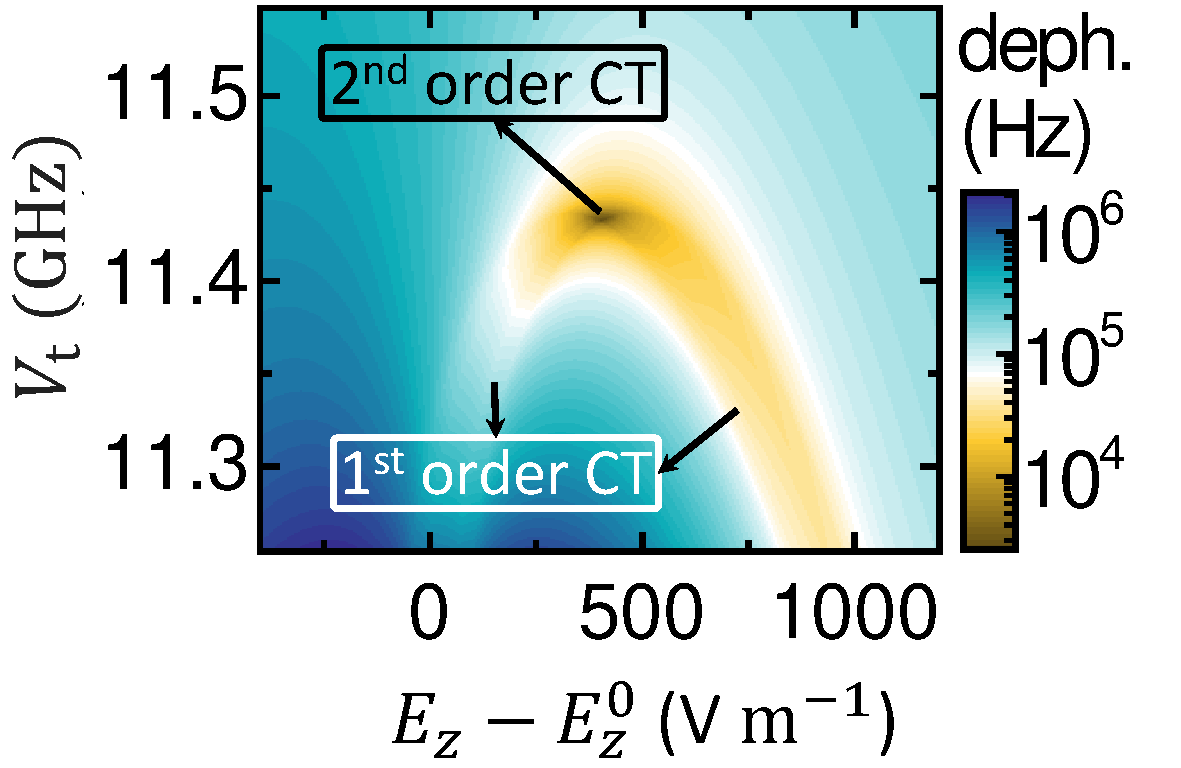
\includegraphics[width=0.65\columnwidth]{polished/ff_dephasing.pdf}
	\caption[Flip-flop dephasing]{\textbf{Flip-flop dephasing} Estimated flip-flop qubit dephasing rate, assuming electric field noise $E_{z, \rm rms}^{\rm noise}=100$~V~m$^{-1}$.}
	\label{fig:ff_dephasing}
\end{figure}

The rates can be as low as $1/T_2^{\ast} \approx 3$~kHz when at the second order clock transition. This is comparable to the dephasing of $1/T_2^{\ast} \approx 1$~kHz due to magnetic noise in our qubits \cite{Muhonen2014}. 

\paragraph{Relaxation}

Relaxation can also inhibit qubit performance. In silicon bulk donors the electron spin lattice relaxation time is $T_1\ll 1\,$s due to very weak coupling between the phonons and the spins. However, according to Ref. \cite{Boross2016},  for the charge and the flip-flop qubit the difference in valley population between the interface and donor state causes a potential energy difference that leads to an effective electron-phonon coupling and to relaxation,even for a uniform phonon-induced relaxation. Basically, the relaxation is "valley-enhanced" due to the non-trivial valley structure of the electron-phonon interaction. The charge qubit relaxation rate is $1/T_{1,c}\approx 0.49\,$MHz at the ionization point and increases with higher $\epsilon_0$. 
In the dispersive regime $\delta_{so}\gg g_{so}$ the flip-flop relaxation directly relates to the charge qubit relaxation. It is equal to the amount of charge excited state in the flip-flop eigenstates times the charge qubit relaxation rate we gives

\begin{equation}\label{eq:T1ff}
{1}/{T_{1,\rm ff}}=\left({g_{\rm so}}/{\delta_{\rm so}}\right)^2/{T_{1,\rm o}},
\end{equation}
\begin{equation}\label{eq:T1o}
{1}/{T_{1,\rm c}}=\Theta\epsilon_{\rm o}{V_t}^2,
\end{equation}
where $T_{1,\rm c}$ is the charge qubit lifetime and $\Theta\approx2.37\times10^{-24}~{\rm s}^2$ is determined by the silicon crystal properties \cite{Boross2016}.

\begin{figure}[h]
	\centering
	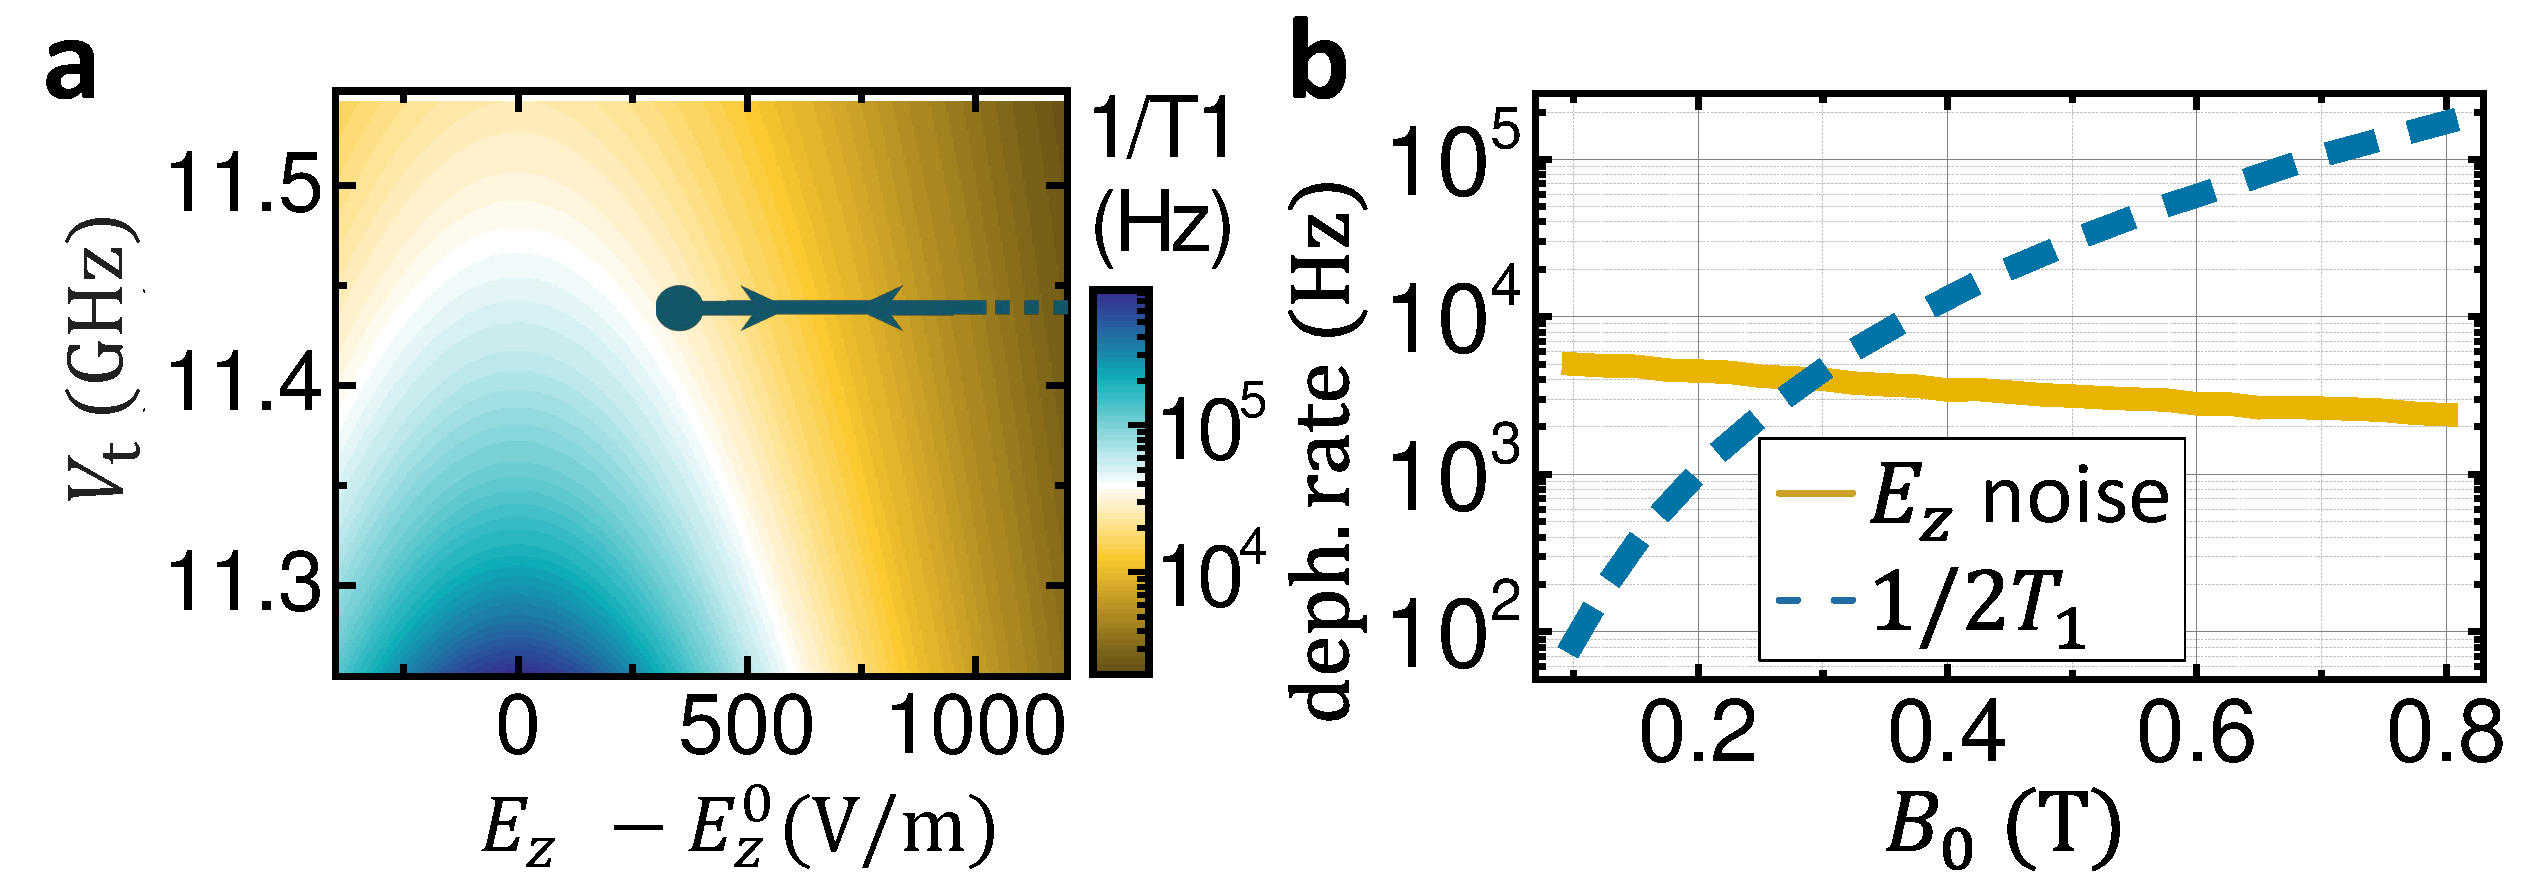
\includegraphics[width=1\columnwidth]{polished/ff_T1.pdf}
	\caption[Flip-flop relaxation rate]{\textbf{Flip-flop relaxation rate. a }Flip-flop qubit relaxation rate, with arrows indicating the adiabatic path used for $z$-gates. \textbf{b} Flip-flop qubit dephasing rate due to $E_z$ noise and relaxation, at $2^{\rm nd}$-order CTs for each $B_0$.}
	\label{fig:T1}
\end{figure}

Figure \ref{fig:T1}a) shows the flip-flop relaxation rate depending on the tunnel coupling and the applied electric field. The larger the detuning, the smaller is the component of admixed excited eigenstate $\ket{e\downarrow\Uparrow}$ and consequently the relaxation. At our proposed operating point at the second order clock transition, the relaxation rate is ${1}/{T_{1,\rm ff}}\sim 10\, $kHz. This indicated that the qubit dephasing will be relaxation limited $1/T_2^*=1/2T_1$. However, the relaxation rate depends on the external magnetic field with the power-law relation $1/T_{1,\rm{ff}}\sim B^3$. Thus reducing the magnetic field, suppresses the relaxation strongly. Figure \ref{fig:T1}b) show the dephasing due to electric noise and relaxation. We find that for $B_0<0.3\,$T, the dephasing is no longer $T_1$ dominated. 


\paragraph{Tunnel coupling tuning}

Tuning the flip-flop qubit, e.g. into a clock transition, requires the ability to tune the tunnel coupling $V_t$. $V_t$ is difficult to control at the fabrication stage, given its exponential dependence on donor depth, together with oscillations at the atomic scale \cite{Calderon2008} arising from a similar valley interference effect as the one afflicting the exchange interaction \cite{Koiller2002}. 

Ion-implanting a donor at $z_d \approx 15$~nm below the interface happens with a vertical uncertainty of order $\pm 10$~nm (ref.~\cite{Donkelaar2015}), resulting in more than 2 orders of magnitude uncertainty in $V_t$ (ref.~\cite{Calderon2008}). Therefore, it is crucial to implement a method to tune $V_t$ \emph{in situ}. A possible solution is to displace the location of the interface wavefunction laterally, which in turn modifies the overlap between the donor and interface wavefunctions and therefore reduces $V_t$. This can be done by adding two gates on either side of the top gate which pulls the donor electron to the interface (Fig.~\ref{fig:Vt_tuning}a)), in such a way that a relative voltage between the gates can modify the interface lateral potential landscape. 

\begin{figure}[h]
	\centering
	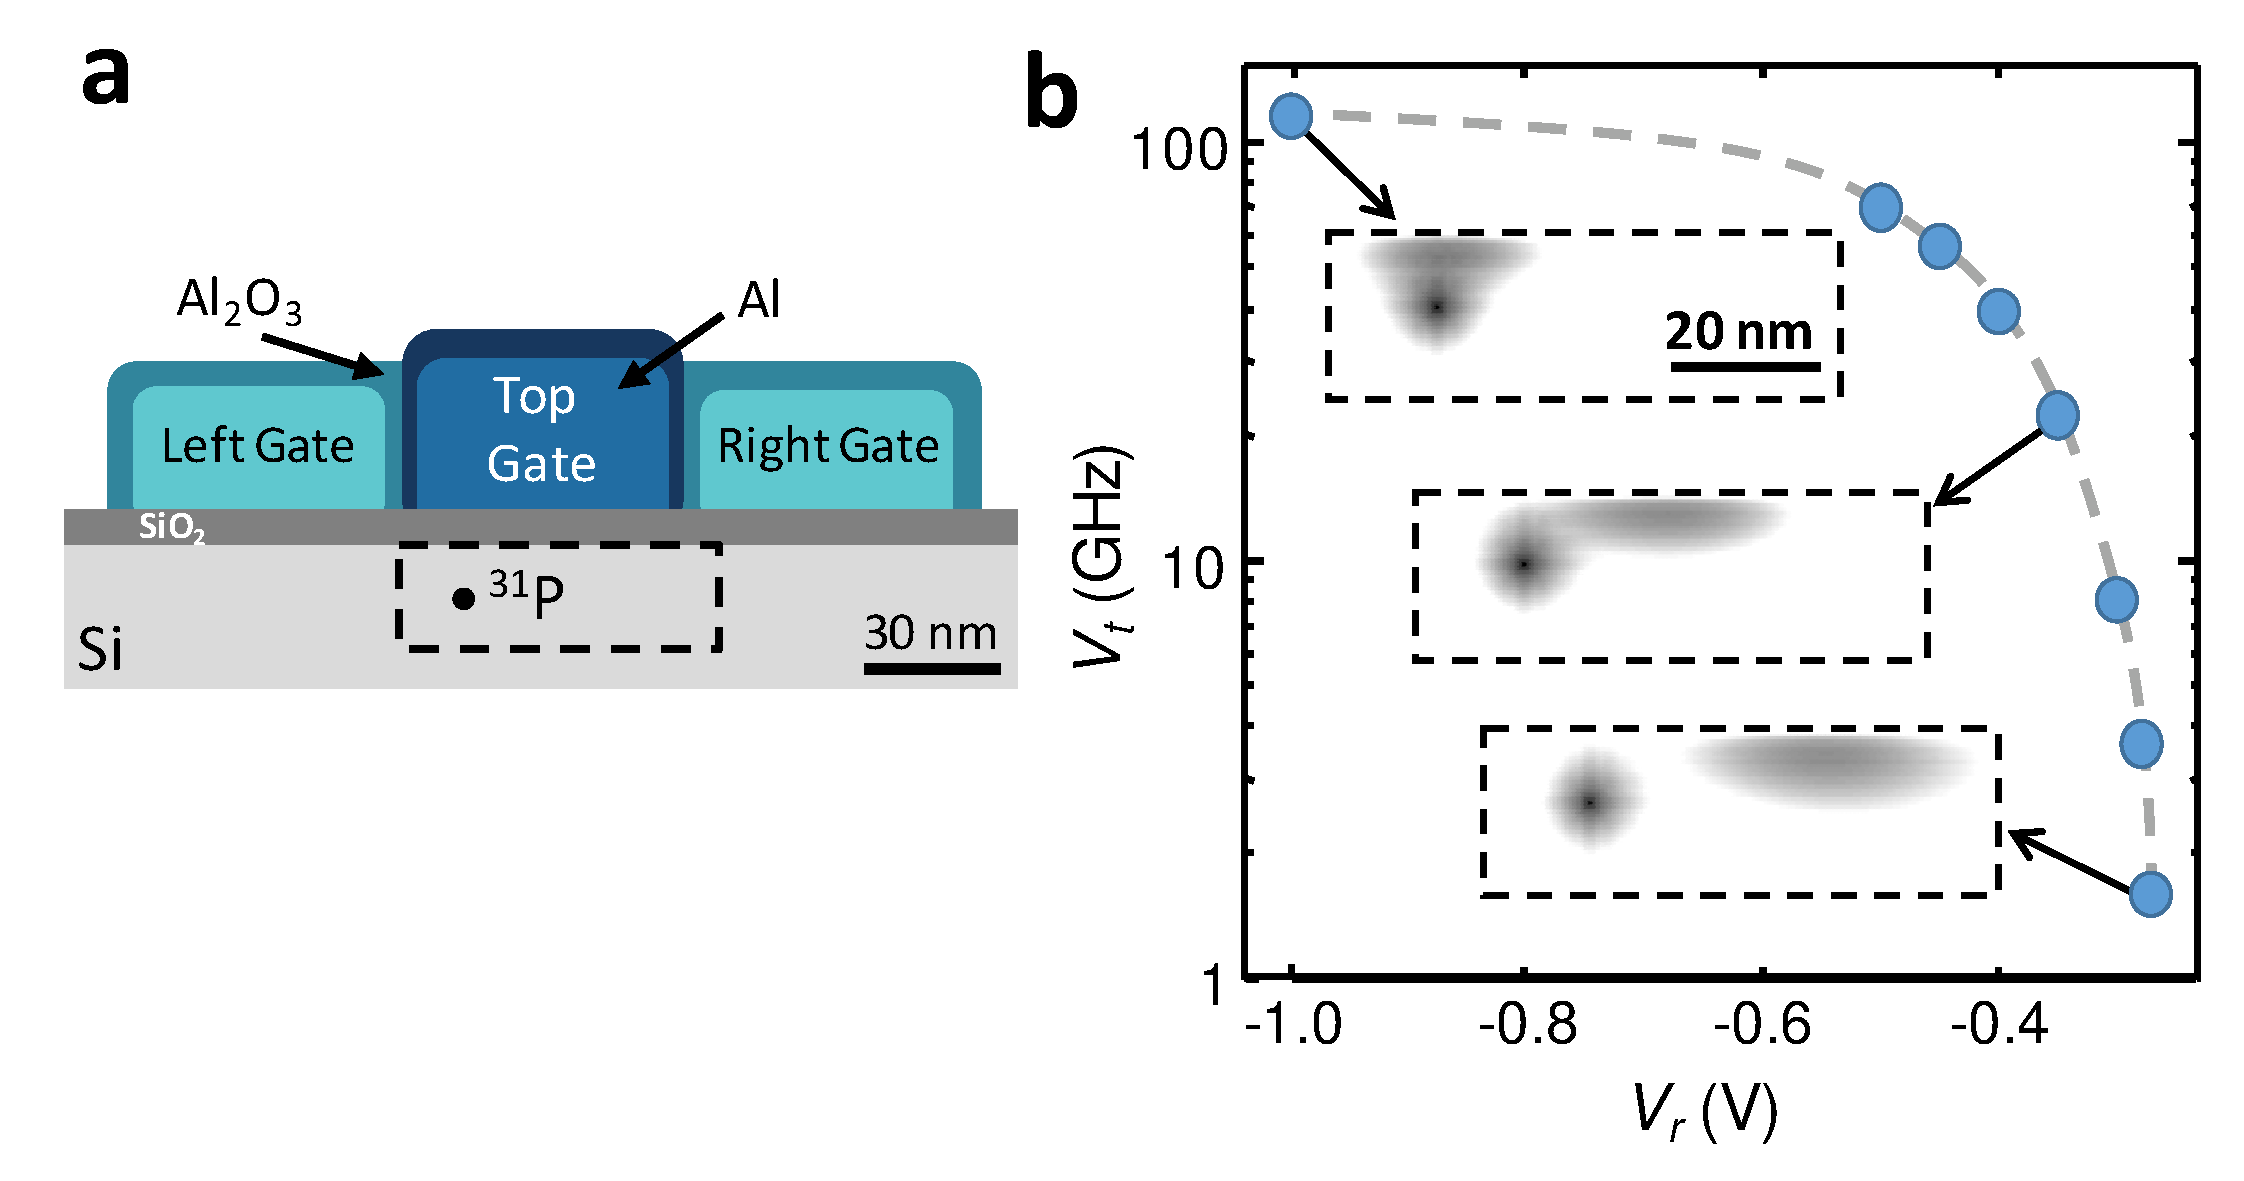
\includegraphics[width=0.8\columnwidth]{polished/Vt_tuning}
	\caption[Tunnel coupling tuning]{\textbf{Tunnel coupling tuning. a} Device structure to tune the tunnel coupling $V_t$ of the charge qubit by applying voltages. Scale bar is 30 nm. 
		\textbf{b}, $V_t$ as a function of right gate voltage, calculated using a finite element Poisson solver (Synopsis\textsuperscript{\textregistered} TCAD) and atomistic tight biding (NEMO-3D, ref.~\cite{Klimeck2007}). The insets illustrate the NEMO-3D wavefunctions inside dashed region in \textbf{f}, for three right gate voltages $V_r=-1$, $-0.35$ and $-0.27$~V. The left gate voltage is $V_l=-0.5$~V for all the simulations, and the top gate is biased such that the position of the electron is in between the donor and interface. Scale bar is 20 nm. The donor is assumed to be $z_d=9.2$~nm below the Si/SiO$_2$ interface.}
	\label{fig:Vt_tuning}
\end{figure}

This gate stack is identical to the well-established scheme for the confinement of single electrons in Si quantum dots \cite{Veldhorst2014}. This technique allows $V_t$ to be reduced by at least 2 orders of magnitude (Fig.~\ref{fig:Vt_tuning}b)), therefore circumventing the uncertainty in donor depth and $V_t$ arising from ion-implantation.

Note that, when moving the interface wavefunction laterally to tune $V_t$, the electric dipole acquires some horizontal component. In this case, the detuning noise is caused by the noise component along the donor-interface states direction. At the same time, horizontal noise will also have an effect, albeit minimal, in gate performance. For the parameters at which $V_t\approx 10$~GHz in Fig.~\ref{fig:Vt_tuning}, $10~\mu$V r.m.s. lateral noise would cause less than 0.01\% uncertainty in the dipole size, therefore causing negligible gate errors. The same noise causes less than 1\% uncertainty in $\delta_{\rm so}$ (and therefore in gate time), which translates into maximum $10^{-4}$ errors due to gate time jitter, and maximum $\sim10^4$~Hz extra dephasing due to dispersive shifts (Eq. \ref{eq:Dorb}).

\paragraph{Adiabatic phase control}

To incorporate flip-flop qubits in a quantum processor, the presence of slow dephasing regions is important to control the qubit phase with high fidelity. Therefore, idle qubits are decoupled from electric fields by fully displacing the electron either to the interface or to the donor to minimize dephasing. Operations are performed close to the ionization point. 
Consequently, we need to displace the electron, which in turn changes its precession frequency (Fig.~\ref{fig:ff_energy}). As a result, the accumulated phase must be corrected after quantum operations. This is optimally done by moving the electron to the $2^{\rm nd}$-order clock transition, therefore minimizing dephasing errors. At this point, the flip-flop qubit phase precesses $\sim\Delta_\gamma\gamma_e B_0/2-D_{\rm orb}\sim\ $GHz faster than its idle point, and therefore any phase correction in a $2\pi$ period can be applied within tens of ns. The dephasing rate at the clock transition, on the order of a few kHz, would cause very small errors ($<10^{-4}$). However, while moving the electron from the interface towards the donor, the flip-flop qubit goes through regions of fast dephasing (Fig.~\ref{fig:ff_dephasing}), and therefore this operation has to be performed as quickly as possible. It also has to be slow enough as to avoid erros due to non-adiabaticity, which include \textit{e.g.} leakage to unwanted high-energy states. These errors depend on the adiabatic factor $K$, which quantifies the fractional rate of change of the system's eigenstates (the higher the value of $K$, the more adiabatic and slower is the process). $K$ is defined, in units of rad/s, as

\begin{equation} \label{eq:K_def}
K=\left|\frac{\omega_{\rm eff}}{\dot{\alpha}}\right|\gg1,
\end{equation}

given a time-dependent Hamiltonian in a two-dimensional Hilbert space, 

 \begin{equation}
\mathcal{H}_2=\Delta(t)\sigma_z+\Omega(t)\sigma_x,
\end{equation}

where $\omega_{\rm eff}=\sqrt{\Delta^2+\Omega^2}$ is the instantaneous transition angular frequency between eigenstates, and $\dot{\alpha}$ is the rate of change of the orientation of $\omega_{\rm eff}$ ($\alpha=\arctan{(\Omega/\Delta)}$) \cite{Garwood2001}. 

It follows from Eq.~\ref{eq:K_def} that

\begin{equation} \label{eq:K_appl}
K=\frac{\left(\Delta^2+\Omega^2\right)^{3/2}}{|\dot{\Delta}\Omega-\dot{\Omega}\Delta|}\gg1,
\end{equation}

We use eq. \eqref{eq:K_appl} to determine the incremental sweep time steps in an adiabatic process to 

\begin{equation} \label{eq:dtK}
dt=K\frac{|d\Delta\cdot\Omega-d\Omega\cdot\Delta|}{\left(\Delta^2+\Omega^2\right)^{3/2}}
\end{equation}

where $d\#$ signifies incremental steps in $E_z$.
Although the transition process involves multiple levels, we applied Eq.~\ref{eq:K_appl} as an approximation of adiabaticity. This was confirmed to be always valid by checking that the leakage errors were kept below a target level.
We use $\Delta_{\rm c}=\pi e(E_z - E_z^0)d/h$ and $\Omega_{\rm c}=\pi V_t$ to find $K_{\rm c}$ for the charge qubit, and $\Delta_{\rm so}=\pi\delta_{\rm so}$ and $\Omega_{\rm so}=2\pi g_{\rm so}$ to find $K_{\rm so}$ for the spin-charge coupling.
 For a chosen adiabatic factor $K$, we then find $E_z(t)$ by satisfying the condition $\min(K_{\rm so},K_{\rm c})=K$.

\begin{figure}[h]
	\centering
	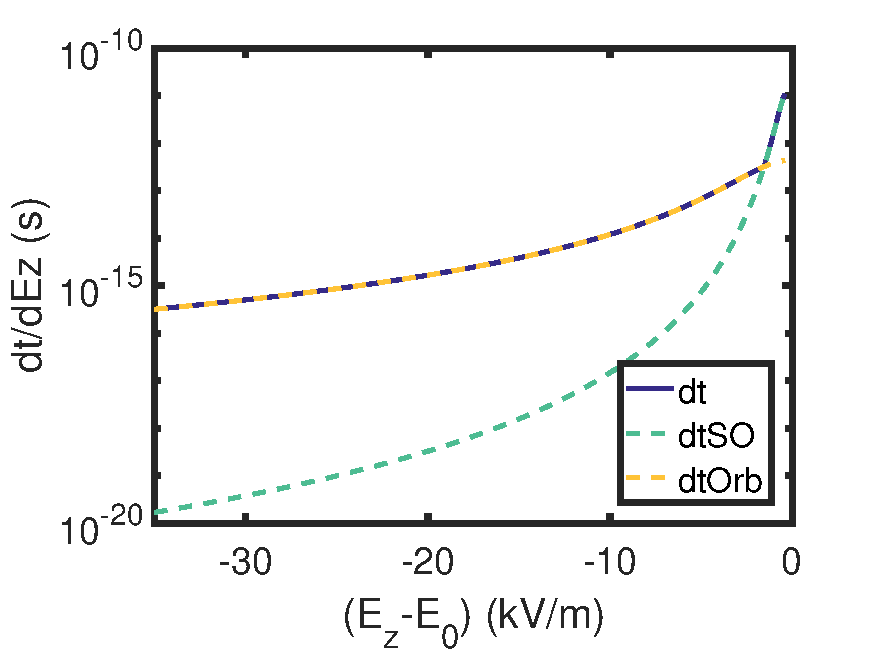
\includegraphics[width=0.8\columnwidth]{polished/adiabatic.pdf}
	\label{fig:z-gate_K}
	\caption[Z-gate adiabaticity time step for each electric field $E_z$]{\textbf{Z-gate adiabaticity time step for each electric field $E_z$}. Time step for each electric field $E_z$ that full fills the adiabaticity criterion from eq. \eqref{eq:K_appl}.}
\end{figure}

\begin{figure}[h]
	\centering
	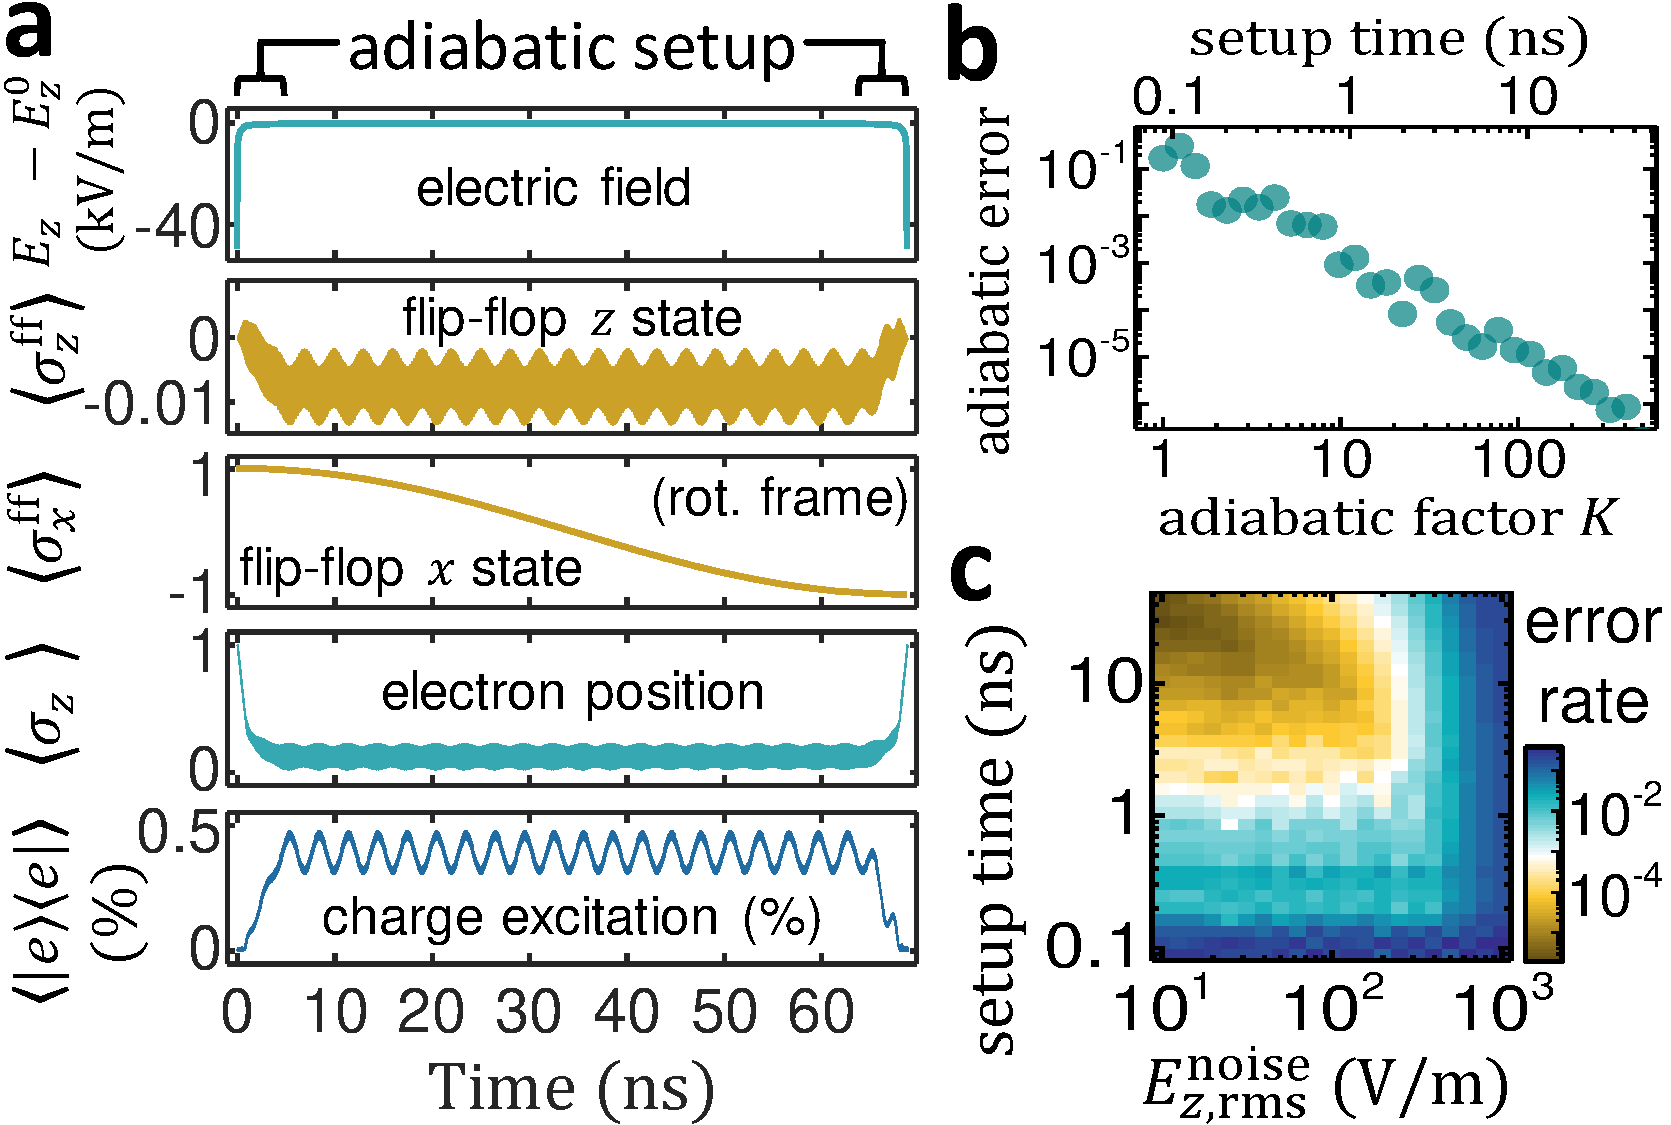
\includegraphics[width=0.9\columnwidth]{polished/z-gate.pdf}
	\caption[High-fidelity adiabatic $z$-gates]{\textbf{High-fidelity adiabatic $z$-gates}.
		\textbf{a}, Time-evolution of an adiabatic  ($K=50$) $\pi$ $z$-gate on state $\ket{g}\otimes(\ket{\downarrow\Uparrow}+\ket{\uparrow\Downarrow})/\sqrt{2}$, showing applied electric field and flip-flop/charge states. Outer brackets denote the expectation value of an operator. $\sigma_z^{\rm ff}=\ket{\uparrow\Downarrow}\bra{\uparrow\Downarrow}-\ket{\downarrow\Uparrow}\bra{\downarrow\Uparrow}$ and $\sigma_x^{\rm ff}=\ket{+_x^{\rm ff}}\bra{+_x^{\rm ff}}-\ket{-_x^{\rm ff}}\bra{-_x^{\rm ff}}$, where $\ket{+_x^{\rm ff}}=\left(\ket{\uparrow\Downarrow}+\exp{\left(-i2\pi\epsilon_{\rm ff}^{t=0}\right)}\ket{\downarrow\Uparrow}\right)/\sqrt{2}$ and $\ket{-_x^{\rm ff}}=\left(\ket{\uparrow\Downarrow}+\exp{\left(-i2\pi\epsilon_{\rm ff}^{t=0}-i\pi\right)}\ket{\downarrow\Uparrow}\right)/\sqrt{2}$. 
		\textbf{b}, $\pi$ $z$-gate leakage error for different adiabatic setup times, which are set by the factor $K$.
		\textbf{c}, $\pi$ $z$-gate error due to quasi-static $E_z$ noise, at the $2^{\rm nd}$-order CT at $B_0=0.4$~T, for different noise amplitudes and adiabatic setup times.}
	\label{fig:z-gate}
\end{figure}



In Fig.~\ref{fig:z-gate}a we plot the time dynamics of an initial state $\ket{g}\otimes(\ket{\downarrow\Uparrow}+\ket{\uparrow\Downarrow})/\sqrt{2}$ while sweeping $E_z$ adiabatically to move the electron from the interface to the $2^{\rm nd}$-order clock transition and back, in order to realize a $\pi$ $z$-gate. Setting $K=50$ eq. \ref{eq:dtK} gives an initial adiabatic setup consisting of a fast sweep (0.8~ns), allowed by the large charge qubit splitting when $E_z \gg E_z^0$, followed by a slower sweep (3.5~ns), limited by the proximity of excited charge states to the flip-flop qubit when $E_z \approx E_z^0$. Figure \ref{fig:z-gate_K} illustrates shows the calculated adiabatic sweep. The electron then remains at the clock transition for 60~ns to perform the gate to correct for the phase shift, according to 
\begin{equation}
t_{\pi}=\frac{\pi/2-\int_{t_0}^{t_{end}} \nu(E_z(t))-\nu(E_z(t_0))dt}{\nu (E_z(t_{end}))-\nu(E_z(t_0))}
\end{equation} 
where $t_{end}=4.3\,$ns. Afterwards we move it adiabatically back to the interface. We calculate the expectation values for the flip-flop z-state $\langle \sigma_z^{ff}\rangle$, the flip-flop x-state $\langle \sigma_x^{ff}\rangle=\ket{+_x^{\rm ff}}\bra{+_x^{\rm ff}}-\ket{-_x^{\rm ff}}\bra{-_x^{\rm ff}}$, where $\ket{+_x^{\rm ff}}=\left(\ket{\uparrow\Downarrow}+\exp{\left(-i2\pi\epsilon_{\rm ff}^{t=0}\right)}\ket{\downarrow\Uparrow}\right)/\sqrt{2}$ and $\ket{-_x^{\rm ff}}=\left(\ket{\uparrow\Downarrow}+\exp{\left(-i2\pi\epsilon_{\rm ff}^{t=0}-i\pi\right)}\ket{\downarrow\Uparrow}\right)/\sqrt{2}$, the electron position $\langle \sigma_z\rangle$ and the charge qubit excitation $\langle \ket{e}\bra{e}\rangle$ by determining the time evolved eigenstates of our system Hamiltonian 

\begin{equation}
\ket{\psi(t)}=e^{-i H t/\hbar}\ket{\psi(t_0)}
\end{equation}

where $\langle \#\rangle=\bra{\psi(t)}\#\ket{\psi(t)}$ (fig. \ref{fig:z-gate}). Indeed during the 69~ns the flip-flop phase $\pi$-gate is performed while keeping both the flip-flop and charge excitation minimal. Fast oscillations between the charge and flip-flop states are due to small deviations from perfect adiabaticity. 

The adiabatic errors (without noise) of an adiabatic unitary process $U_{\rm ideal}$, expressing leakage to other states, can be calculated by averaging the fidelity of the actual process $U$ over a set of initial states $\ket{j}$,

\begin{equation}\label{eq:adError}
{\rm Adiabatic~error}=1-\sum\limits_{\ket{j}}{\left|\bra{j}U^\dagger U_{\rm ideal}\ket{j}\right|^2/N_j},
\end{equation}

where $N_j$ is the number of initial states. For this 1-qubit gate, we choose $\ket{j}=\{\ket{g\downarrow\Uparrow}_e,\ket{g\uparrow\Downarrow}_e,(\ket{g\downarrow\Uparrow}_e+\ket{g\uparrow\Downarrow}_e)/\sqrt{2},(\ket{g\downarrow\Uparrow}_e+i\ket{g\uparrow\Downarrow}_e)/\sqrt{2}\}$ and $N_j=4$. 

These errors can be controlled with the factor $K$, which determines the setup time (see Fig.~\ref{fig:z-gate}b).

Quasi-static $E_z$ noise can increase errors, due to dephasing (Fig. \ref{fig:z-gate}c). At realistic noise levels (100~V~m$^{-1}$), the gate error rate is found to be $<10^{-4}$. Similar error levels arise due to relaxation, which remains below $3\cdot 10^4$~Hz (Fig.~\ref{fig:T1}).\\

Note that the presence of clock transitions does not affect the ability to use $E_{\rm ac}$ to resonantly drive the qubit, since the transverse term $A(E_z)$ still responds fully to the electric field (this is similar to the case of magnetic clock transitions, e.g. in Si:Bi \cite{Wolfowicz2013}).


\section{Electric drive}

\begin{figure}[h]
	\centering
	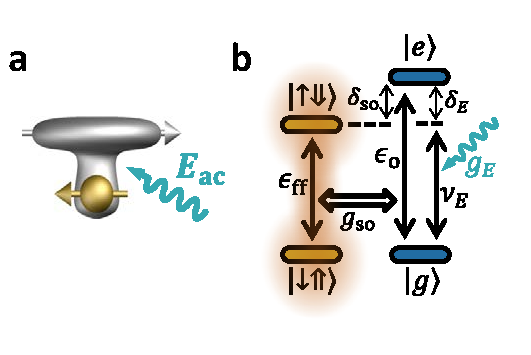
\includegraphics[width=0.7\columnwidth]{polished/elecDrive.pdf}
	\caption[Electric drive of the flip-flop qubit]{\textbf{Electric drive of the flip-flop qubit. a}, Spatial representation and \textbf{b}, level diagram, for electrical drive of a flip-flop qubit, showing partially ionized electron wavefunction and spin arrows.}
		\label{fig:elec_drive}
\end{figure}


We can achieve high-fidelity one-qubit $x(y)$-gates with an electric drive of the flip-flop qubit as illustrated in figure \ref{fig:elec_drive}(a).  The fastest 1-qubit gates are obtained when the electron is around the ionization point, where $\partial A/\partial E_z$ is maximum (Fig. \ref{fig:hfchange}). A vertical oscillating electric field of amplitude $E_{\rm ac}$ is applied in resonance with the flip-flop qubit, \textit{i.e}, $\nu_E=\epsilon_{\rm ff}$. This renders $\mathcal{H}_A(t)$ time-dependent with a component $A_{\rm ac}\cos{\left(2\pi\nu_E t\right)}$, resulting in a coupling rate

\begin{equation}\label{eq:gE_Aac}
g_E^{\rm ff}=A_{\rm ac}/4.
\end{equation}

The oscillation strength $A_{ac}$ depends on the driving electric field, described by the Hamiltonian 

\begin{equation}
H_{E}=E_{ac}\cos(2\pi\nu_E t)\sigma_z
\end{equation}
where $E_{ac}$ is the electric drive amplitude.  The coupling of this electric field to the charge qubit is then determined by 

\begin{eqnarray} \label{eq:g_E}
g_{E}& =& \bra{g}H_{E}\ket{e}\\
 &=& \frac{e E_{\rm ac} d}{4h}\bra{g}\sigma_z\ket{e}\\
 & = &\frac{e E_{\rm ac} d}{4h}\frac{V_t}{\epsilon_{\rm o}}.
\end{eqnarray}

This coupling rate corresponds to half the Rabi frequency in the one-photon limit. Furthermore, in every case of resonant driving we assume a linearly polarized field, resulting in a Rabi frequency that equals half the dipole matrix element times the driving field amplitude (rotating-wave approximation). This explains the factors of 4 appearing in all the formulas for coupling rates.

Figure \ref{fig:drive_levels} (b) portraits the energy level diagram for the electric drive.  A large detuning $\delta_{\rm so}\gg g_{\rm so}$ (Fig. \ref{fig:1-qubit}b) between the charge and flip-flop qubit ensures the least amount of the charge excited state $\ket{e}$ in the flip-flop qubit eigenstates, minimizing qubit relaxation via charge-phonon coupling. The flip-flop qubit is still driven, via a second-order process, at a rate (half-Rabi frequency) given by second order perturbation theory to:
 
 \begin{eqnarray} \label{eq:g_E_ff}
g^{\rm ff}_{E}&=&\frac{\left| \langle \uparrow\Downarrow g|H\ket{e\downarrow\Uparrow}\langle e\downarrow\Uparrow|H\ket{g\uparrow\Downarrow}\right|}{E_{e\downarrow\Uparrow}-E_{g\uparrow\Downarrow}} ???? \\
&=&\frac{g_{\rm so}g_{E}}{2}\left(\frac{1}{\delta_{\rm so}}+\frac{1}{\delta_E}\right),
\end{eqnarray}


where $\delta_E=\nu_E-\epsilon_{\rm o}$.
Equation \ref{eq:g_E_ff} provides another explanation of why the fastest 1-qubit gates are obtained when the electron is at the ionization point: $\delta_{\rm so}$ and $\delta_E$ are minimum ($\epsilon_{\rm o}$ is minimum), and $g_{\rm so}$ and $g_E$ are maximum (Eqs. \ref{eq:g_so} and \ref{eq:g_E}).

\begin{figure}[h]
	\centering
	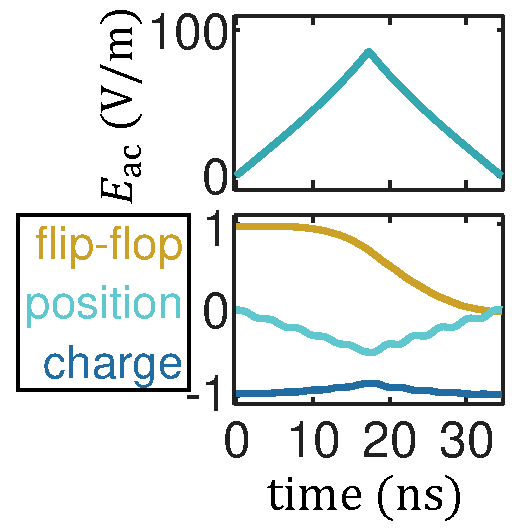
\includegraphics[width=0.4\columnwidth]{polished/adiabaticEdrive.pdf}
	\caption[Adiabatic flip-flop electric drive]{\textbf{Adiabatic flip-flop electric drive} Time-dependent adiabatic drive amplitude and qubit dynamics of a $\pi/2$ $x$-gate, for $K=30$, $B_0=0.4$~T, $E_z=E_z^0$ and $V_t=11.5$~GHz. Right plot shows flip-flop z state, $\langle\sigma_z^{\rm ff}\rangle$, electron position, $\langle\sigma_z\rangle$, and charge qubit state, $\langle\ket{e}\bra{e}-\ket{g}\bra{g}\rangle$.}
		\label{fig:adEdrive}
\end{figure}

The electrical drive can cause some excitation of the charge qubit. It is therefore convenient to turn $E_{\rm ac}$ on/off adiabatically to make sure the charge is de-excited at the end of the gate. Figure \ref{fig:adEdrive} shows the $E_{\rm ac}$ time evolution needed for a $\pi/2$ $x$-gate. The adiabatic increase of $E_{ac}(t)$ is calculated with eq. \eqref{eq:K_appl} with $\Delta_E=\pi\delta_E$ and $\Omega_{E}=2\pi g_E$ where we have assumed an adiabatic factor $K=30$, sufficient for leakage errors $<10^{-3}$. Once $E_{\rm ac}(t)$ has been determined, we employ Floquet theory to calculate time evolution of the Hamilonian which now changes with every time step.  

Floquet theory says that semi-classical theory provides results that are equivalent to full quantum theory in cases of driving fields interacting with a (qubit) system when fluctuations in the phonon number can be neglected \cite{floquet}. For a periodic Hamiltonian $H(t)=H(t+T)$ with $T$ we define the time propagator as 

\begin{equation}
\ket{\psi(t)}=K(t,t_0)\ket{\psi(t_0)},
\end{equation}
with $K(t_0,t_0)=1$. We can use the propagator over a full period $K(T,0)$ to construct a time evolution over many multiples $n$ of the fundamental period
\begin{equation}
K(nT,0)=[K(T,0)]^n
\end{equation}

This can be used when de-constructing the adiabatic evolution into many small time steps which result in the final time-evolved operator $H$. This can then be used to calculate the expectation values of flip-flop z-state $\langle \sigma_z^{ff}\rangle$, the electron position $\langle \sigma_z\rangle$ and the charge qubit state $\langle \ket{e}\bra{e}-\ket{g}\bra{g}\rangle$. 
In our $\pi/2$ $x$-gate, $E_{ac}$ increases steadily until a $\pi/4$ rotation is completed, after which $E_{\rm ac}$ is gradually switched off to achieve the gate. Meanwhile, an average 4\% excitation of the charge qubit causes a $\sim4\cdot 10^4$~Hz relaxation rate of the encoded quantum state (Eq. \ref{eq:T1o}), or error levels close to $10^{-3}$. 

\begin{figure}[h]
	\centering
	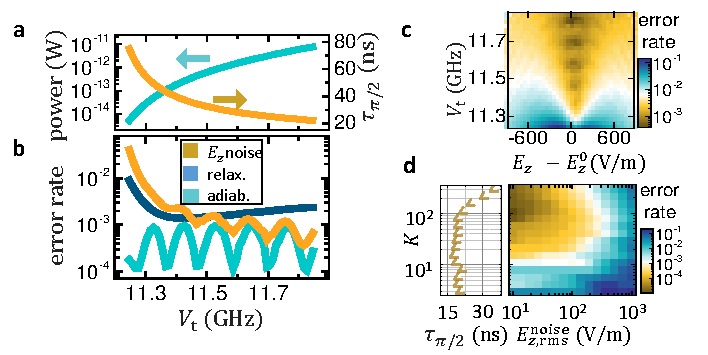
\includegraphics[width=1\columnwidth]{polished/adiabaticError.pdf}
	\caption[Adiabatic gate errors]{\textbf{Adiabatic gate errors. a} Averaged drive power and gate time for the parameters $K=30$, $B_0=0.4$~T, $E_z=E_z^0$ and $V_t=11.5$~GHz. For the same parameters, \textbf{b} the error rates for different $V_t$. To estimate the drive power, we assumed a 50~$\Omega$ line in which a $1~{\rm \mu V}$ AC voltage produces a 10~V~m$^{-1}$ AC vertical electric field.
		\textbf{c}, Estimated flip-flop qubit $\pi/2$ $x$-gate error due to quasi-static noise with amplitude $E_{z, \rm rms}^{\rm noise}=100$~V~m$^{-1}$.
		\textbf{d}, Dependence of the gate error rate on the electric noise r.m.s. amplitude and adiabatic factor K (which sets the gate time).}
	\label{fig:adError}
\end{figure}

We then investigate in figure \ref{fig:adError}(a) how the total $\pi/2$ $x$-gate errors depend on the biasing of the electron wavefunction by calculating the adiabatic error from eq. \eqref{eq:adError} and the error from quasi-static $E_z$ noise from
 
\begin{equation}\label{eq:noiseError}
{\rm Noise~error}=1-\sum\limits_{n,\ket{j}_n}{\left|\bra{j}_nU_n^\dagger U_{n,\rm ideal}\ket{j}_n\right|^2/(N_jN_n)}
\end{equation}
where $\ket{j}=\{\ket{g\downarrow\Uparrow}_e,\ket{g\uparrow\Downarrow}_e,(\ket{g\downarrow\Uparrow}_e+\ket{g\uparrow\Downarrow}_e)/\sqrt{2},(\ket{g\downarrow\Uparrow}_e+i\ket{g\uparrow\Downarrow}_e)/\sqrt{2}\}$ and $N_j=4$. 

%1. Find adiabatic shape Eac(t)
%2. find time evolved H(t) with Eac(t) through Floquet
%3. Find time evolved states psi with H(t)
%4. Find fideilities with H(t) and Psi(t)

 At the ionization point, $E_z=E_z^0$, error levels close to $10^{-3}$ are found over a wide range of $V_t$. The $K=30$ choice ensures adiabatic errors $<10^{-3}$ with an oscillatory character typical of adiabatic processes \cite{Oh2013}. At small $V_t$ (and therefore small detuning $\delta_{\rm so}$), the qubit eigenstates contain a substantial amount of charge, causing more errors due to charge-phonon relaxation. Increasing the detuning $\delta_E$ with larger $V_t$ allows for a faster adiabatic sweep and higher powers (Fig.~\ref{fig:adError}(b)), yielding shorter gate times and therefore less errors due to quasi-static noise. Still, the incident power is at least three orders of magnitude lower than the one needed to drive donor electron spin qubits, at the same Rabi frequency, with oscillating magnetic fields \cite{Pla2012,Muhonen2014}.

As Fig. \ref{fig:adError}(a) shows, low error rates are still available away from the ionization point, even though best values are found at $E_z=E_z^0$. This is because our gate times are so fast that dephasing, and therefore CT's, do not play a crucial role. Instead, quasi-static $E_z$ noise cause errors mainly by modulating the driving strength $g_E^{\rm ff}$, causing ``gate time jitter''. Indeed, the gate time is sensitive to the orbital transition frequency $\epsilon_{\rm o}$ (Eq. \ref{eq:g_E_ff}), and therefore gate errors are minimized close to the charge qubit sweet spot (CQSS), where $\partial\epsilon_{\rm o}/\partial E_z=0$ (Fig. \ref{fig:ff_dephasing}).

Finally, as Fig. \ref{fig:adError}(c) shows, lower quasi-static $E_z$ noise can cause less errors, provided that the adiabatic factor $K$ is increased, to reduce leakage errors, up to an optimum value where gate times are still fast as to keep noise errors low. Relaxation errors could also be reduced by reducing $B_0$ (recall Fig.~\ref{fig:T1}).

A number of other noise sources can also affect the qubits. Another source of electric field noise can be the thermal and electrical noise produced by the metallic gates on top of the qubits, and the room-temperature instruments they connect to. An $R=50~\Omega$ resistor at room temperature produces Johnson-Nyquist noise with an r.m.s voltage $\sqrt{4k_BTR\Delta\nu}$. Therefore a quasi-static bandwidth $\Delta\nu\sim10^6$~Hz produces $\sim1~\mu$V voltage noise, which is equivalent to $E_{z,\rm rms}^{\rm noise}\sim10$~V~m$^{-1}$, or errors $<10^{-5}$ (Fig.~\ref{fig:adError}c). Furthermore, because of the very low powers required by the electrically-driven 1-qubit gates and adiabatic shuttling, it is possible to insert abundant low-temperature attenuation along the high-frequency lines, and therefore the relevant temperature for the Johnson-Nyquist noise is well below room temperature. On the other hand, being close to a metallic interface, our qubit will be subject to evanescent wave Johnson noise (EWJN) due to vacuum and thermal fluctuations. Assuming the qubit is $z=15$~nm under aluminum gates at $T=100$~mK ($\sigma=1.4\times10^8$~S~m$^{-1}$ conductivity \cite{Dehollain2013S}), a quasi-static bandwidth $\Delta\nu\approx10^6$~Hz produces \cite{Henkel1999S} $\sqrt{k_BT\Delta\nu/(2z^3\sigma)}\sim0.04$~V~m$^{-1}$ r.m.s. electric field noise, therefore negligible. We conclude that the main source of quasi-static noise will be charge noise with a typical $1/\nu$ spectrum. Consistently with recently measured for Si/SiO$_2$ interfaces \cite{Freeman2016S}, we assume the power spectral density to be $S_{\rm c}(\omega)\approx10^4/(6\omega)$, in units of ${\rm V^2~m^{-2}~rad^{-1}~s}$.

So far we have only considered quasi-static noise. The presence of some residual amount of high-frequency noise could possibly lead to errors while performing quantum operations. Below we discuss these high-frequency sources, finding that they will cause much smaller errors compared to quasi-static noise.

In general, a driven qubit Rabi-oscillates with a decay envelope function given by \cite{Bylander2011S} $\zeta(t)\exp(-\Gamma_Rt)$, where $\zeta(t)$ represents decay due to quasi-static detuning noise and $\Gamma_R$ the exponential Rabi decay rate, which combines the qubit relaxation rate, $\Gamma_1$, the inverse of the gate time jitter due to quasi-static noise, $\Gamma_1^{\Delta}$, the inverse of the gate time jitter due to noise at the drive frequency, $\Gamma_1^{\nu}$, (the last three yield $T_{2\rho}$ in the dressed qubit picture \cite{Laucht2016S}) and the decay rate due to detuning noise at the Rabi frequency, $\Gamma_\Omega$ (which equals the inverse of $T_{1\rho}$ in the dressed qubit picture \cite{Yan2013S,Laucht2016S}).

The effects of $\zeta(t)$, $\Gamma_1$ and $\Gamma_1^{\Delta}$ have already been discussed extensively in this manuscript, with corresponding error levels below $10^{-3}$. We now focus on errors due to high-frequency noise sources, corresponding to decay rates $\Gamma_1^{\nu}$ and $\Gamma_\Omega$.

Vertical (thus parallel to the driving field $E_{\rm ac}$) noise at the qubit resonance frequency ($\sim 10^{10}$~Hz) would cause transitions between the qubit eigenstates -- essentially a spurious excitation/relaxation process driven by noise -- at a rate $\Gamma_1^{\nu}$. This noise can be caused $e.g.$ by charges fluctuating in resonance with the qubit or by voltage noise at the metallic gates. This includes vacuum fluctuations, especially since the qubit frequency is generally higher than the corresponding device temperature. Also, during gate operations, the portion of the noise spectrum %contained within a power-broadened bandwidth $<10^5$~Hz
around the qubit frequency can add incoherently to the external resonant drive, causing the gate time to fluctuate. For the flip-flop qubit, the Rabi decay rate is given by $\Gamma_1^\nu=(\pi/2)(\mu_e^{\rm ff}/\hbar)^2S(2\pi\epsilon_{\rm ff})$, where $\mu_e^{\rm ff}=ed\langle g_{\rm so}/\delta_{\rm so}\rangle$ is the average flip-flop qubit electric dipole moment and $S(2\pi\epsilon_{\rm ff})$ is the noise power spectral density at the qubit angular frequency (in units of ${\rm V^2~m^{-2}~rad^{-1}~s}$). Note that this flip-flop electric dipole is much smaller than the charge dipole, which in turn makes it less susceptible to electrical noise. This happens because, in our gate scheme, the charge dipole is only used as a second-order enabler, and therefore charge excitation is greatly minimized (Figs. \ref{fig:z-gate}a, \ref{fig:1-qubit}c and \ref{fig:iSWAP}a). In case of charge noise, $S_{\rm c}(\omega)=10^4/(6\omega)$, which gives $\Gamma_1^\nu\sim10^4$~Hz. This implies $\pi/2$ $x$-gate errors $\sim10^{-4}$. There could also be vacuum fluctuations of charge traps, which could also generate errors due to relaxation. We do not know of any experimental measurement of such a noise for semiconductor nanostructures. For superconducting charge qubits, it has been found that charge noise increases linearly at frequencies beyond the thermal bath \cite{Astafiev2004S}, which has been explained in terms of two-level coherent charge fluctuators \cite{Shnirman2005S}. If a similar phenomenon afflicts our qubits, those quantum fluctuations will play an important role beyond $\sim2$~GHz (100 mK), implying that, at 10 GHz, relaxation can be up to 25 times faster. This can increase relaxation error rates to $\sim10^{-3}$. In case of Johnson-Nyquist noise, $S_{\rm JN}(\omega)= 2\times10^{14}R\hbar\omega\pi^{-1}(e^{\hbar\omega/k_BT}-1)^{-1}$ (where we have used $\partial E_z/\partial V=10^7~{\rm m^{-1}}$, typical in MOS nanostructures). Because of the very low powers required by the electrically-driven 1-qubit gates ($<1$~pW), it is possible to insert abundant low-temperature attenuation along the high-frequency lines, insuring that the gates are well thermalized, and the noise of the room-temperature electronics greatly attenuated. A noise temperature $T=100$~mK would give $\Gamma_1^\nu<10^4$~Hz, and therefore error rates $<10^{-4}$. Finally, in case of EWJN at $T=100$~mK, the $10^{10}$~Hz part of the spectrum is \cite{Henkel1999S,Poudel2013S} $S_{\rm EW}(\omega)\approx\hbar\omega/(4\pi z^3\sigma)$. This would give $\Gamma_1^\nu<10^4$~Hz, therefore again error rates $<10^{-4}$.

Noise at the Rabi frequency ($\Omega_R>10^{7}$~Hz) causes decay in the Rabi oscillations at a rate $\Gamma_\Omega$. This type of noise feeds into the driven qubit via fluctuations in the detuning between drive frequency and the qubit precession frequency. The decay rate of the flip-flop qubit is given by $\Gamma_\Omega=(\pi/2)(2\pi\sum_{i=x,y,z}\partial\epsilon_{\rm ff}/\partial E_i)^2S(\Omega_R)$. At the low-error operation region of Fig. \ref{fig:1-qubit}f, $\partial\epsilon_{\rm ff}/\partial E_z\sim10^3~{\rm Hz~V^{-1}~m}$ and $\partial\epsilon_{\rm ff}/\partial E_{x,y}\sim10^2~{\rm Hz~V^{-1}~m}$ (from Fig.~\ref{fig:clock}g). $1/\nu$ charge noise gives $\Gamma_\Omega<10^4$~Hz, implying $<10^{-4}$ errors. Johnson-Nyquist noise from room temperature gives $\Gamma_\Omega=3\times10^2$~Hz, whereas EWJN at 100~mK gives $\Gamma_\Omega=2\times10^1$~Hz, therefore producing $<10^{-5}$ and $<10^{-6}$ errors, respectively.


\begin{table}
\centering
\begin{tabular}{|p{1.4in}|p{0.7in}|p{0.7in}|p{0.7in}|} \hline 
 & \multicolumn{3}{|p{2.0in}|}{\textbf{Error levels at different spectral bandwidths}} \\ \hline 
\textbf{Noise source} & Quasi-static\newline ($<$10${}^{6}$ Hz) & Rabi\newline ($\sim 10^{7}$ Hz) & Qubit\newline ($\sim 10^{10}$ Hz) \\ \hline 
1/f vertical ($E_z$) & $10^{-3}$ & $<10^{-4}$ & $10^{-4}$ \\ \hline 
1/f horizontal ($E_{x,y}$) & $10^{-4}$ & $<10^{-5}$ & - \\ \hline 
Charge-phonon\newline relaxation & - & - & $10^{-3}$ \\ \hline 
Johnson-Nyquist & $<<10^{-5}$ & $<10^{-5}$ & $<10^{-4}$ \\ \hline 
EWJN & - & $<10^{-6}$ & $<10^{-4}$  \\ \hline 
\end{tabular}
	\caption[Gate errors for different noise sources]{\textbf{Gate errors for different noise sources} Hyphens indicate non-existent or negligible errors.}
	\label{tab:noise}
\end{table}

We conclude that quasi-static $E_z$ noise and charge-phonon relaxation are the main sources of error and the most deleterious ones for flip-flop qubits. Therefore our analysis is sufficient to provide a reliable estimate of dephasing and gate errors. Indeed, low-frequency noise was found to be the most deleterious one in a hybrid donor-dot qubit in a silicon MOS device \cite{Harvey-Collard2015S}. Finally, note that we do not assume any type of dynamical noise correction or cancellation to be applied, and therefore our calculations are a worst-case scenario. Table \ref{tab:noise} summarizes these results. 

\section{Two-qubit coupling}

To couple two flip-flop qubits, we the electric dipole that naturally arises when a donor-electron wavefunction is biased to the ionization point, due to the fact that a negative charge has been partly displaced away from the positive $^{31}$P nucleus. The electric field produced by this induced dipole in turn, modifies the energy of a nearby donor which is also biased at the ionization point, resulting in a long-range coupling between the two. This is illustrated in figure \ref{fig:dipole}(a).

\begin{figure}[h]
	\centering
	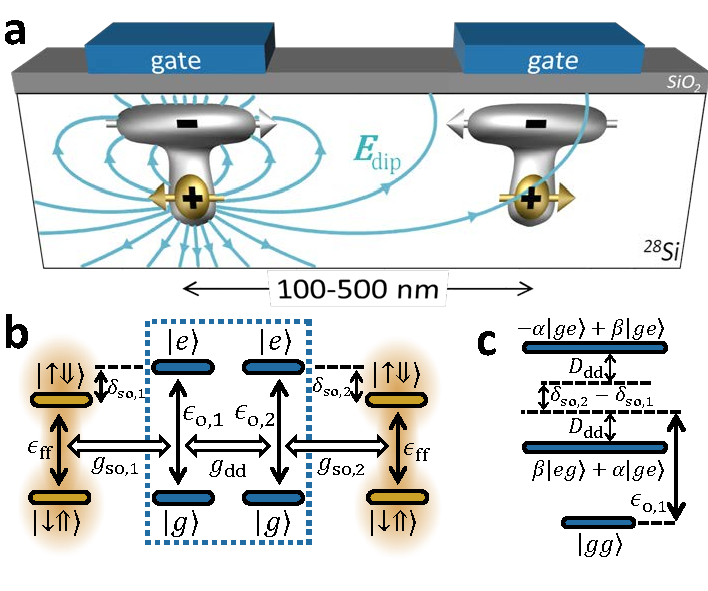
\includegraphics[width=0.8\columnwidth]{polished/2qubit_dipole.pdf}
	\caption[Electric dipole-dipole interactions between two distant flip-flop qubits]{\textbf{Electric dipole-dipole interactions between two distant flip-flop qubits. a}, Device scheme for coupling qubits, showing dipole field lines, $\textit{\textbf{E}}_{\rm dip}$, produced by the dipole on the left.
		\textbf{b}, Level diagram for two-qubit coupling via electric dipole-dipole interaction.
		\textbf{c}, Lowest molecular eigenstates for the two charge qubits inside dashed rectangle in \textbf{b}.}
	\label{fig:dipole}
\end{figure}

The interaction energy between two distant dipoles, $\mu_1$ and $\mu_2$, oriented perpendicularly to their separation $r$ is $V_{\rm dip}=\mu_1\mu_2/(4\pi\varepsilon_r\varepsilon_0r^3)$, where $\varepsilon_0$ is the vacuum permittivity and $\varepsilon_r$ the material's dielectric constant ($\varepsilon_r=11.7$ in silicon)\cite{Ravets2014}. The electric dipole of each donor-interface state is $\mu_i=ed_i(1+\sigma_{z,i})/2$, implying that the dipole-dipole interaction Hamiltonian is:

%\begin{subequations}
\begin{equation} \label{eq:H_dipdip}
\mathcal{H}_{\rm dip}=V_{\rm dd}\left(\sigma_{z,1}\sigma_{z,2}+\sigma_{z,1}+\sigma_{z,2}\right)
\end{equation}
\begin{equation} \label{eq:V_dd}
V_{\rm dd}=\frac{1}{16\pi\varepsilon_0\varepsilon_r h}\frac{e^2d_1 d_2}{r^3}
\end{equation}
%\end{subeq uations}

This electric dipole-dipole interaction is therefore equivalent to a small shift in the equilibrium orbital position of both electrons plus a coupling term between the charge qubits (blue dashed rectangle in Fig. \ref{fig:dipole}b) equal to:

\begin{eqnarray} \label{eq:g_dd}
g_{\rm dd} & = & \bra{e_1g_2}H_{\rm dip, coupling}\ket{g_1e_2}\\
 & = & V_{dd}\bra{e_1}\sigma_{z,1}\ket{g_1}\bra{g_2}\sigma_{z,2}\ket{e_2}\\
 & = &  V_{\rm dd}\frac{V_{t,1}V_{t,2}}{\epsilon_{\rm o,1}\epsilon_{\rm o,2}}
\end{eqnarray}

The strength of the dipole also depends on screening effects.   

\paragraph{Dipole Screening}

Our device topology consists of a SiO$_2$ layer sandwiched between a metal gate and silicon substrate, with the donor embedded in the substrate. In such a topology, the image charges of the donor electron and nucleus will be located above the donor, thereby creating an additional vertical dipole.

\begin{figure}
\centering
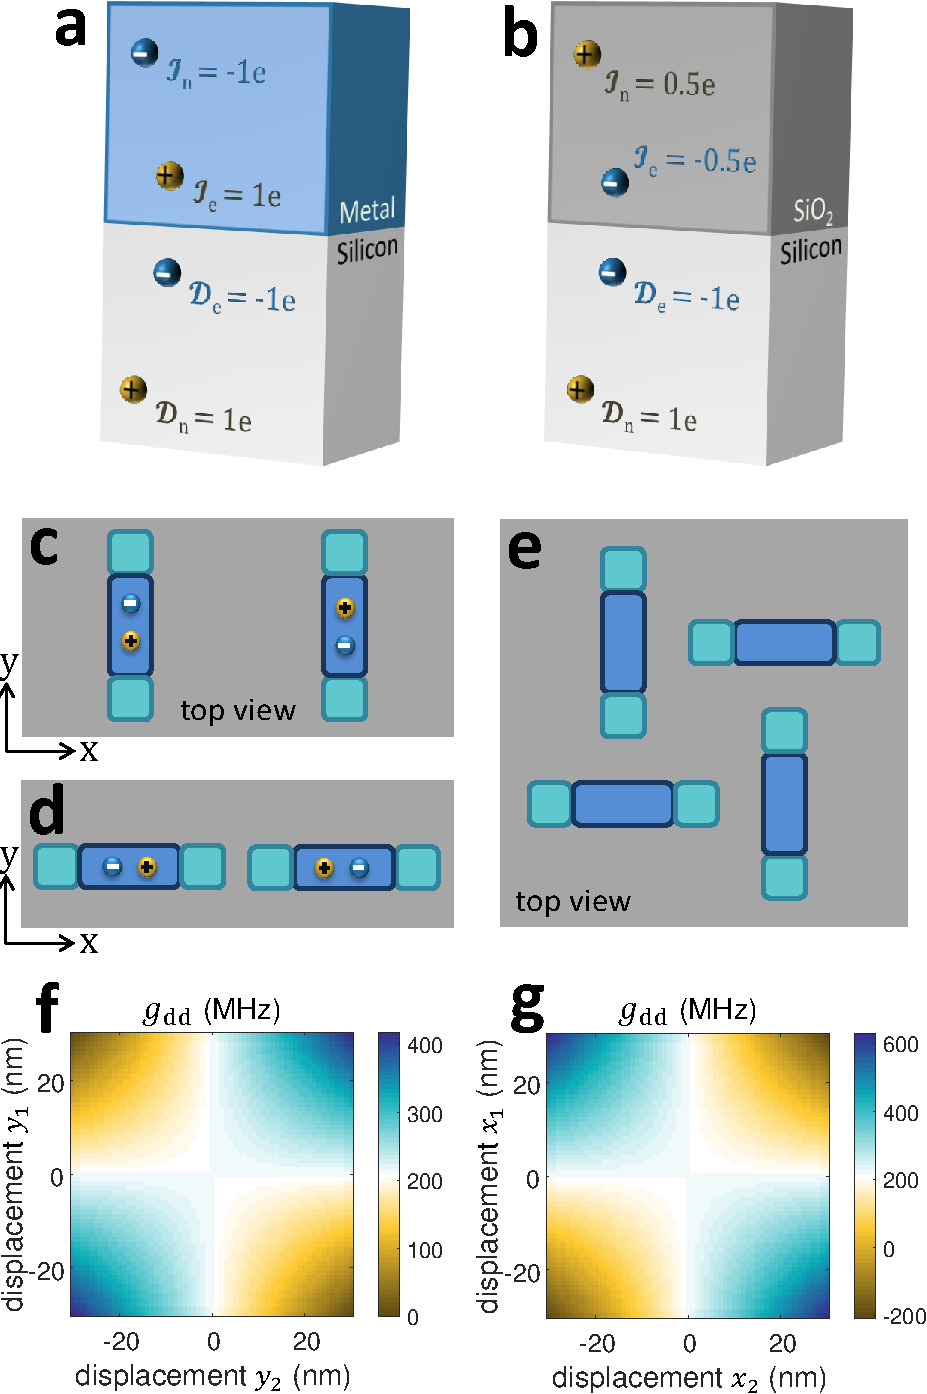
\includegraphics[width=0.7\columnwidth]{polished/image-charges.pdf}
\caption[Screening and image charges]{\textbf{Screening and image charges.} Image ($\mathcal{I}_\mathrm{e}$ and $\mathcal{I}_\mathrm{n}$) charges of the donor electron ($\mathcal{D}_\mathrm{e}$) and nucleus ($\mathcal{D}_\mathrm{n}$) for silicon-metal (\textbf{a}) and silicon-oxide (\textbf{b}) interfaces. The magnitude and polarity of the image charges are given by Supplementary Eq. \ref{eq:ImageCharge}. Schematic top view of two interacting dipoles when the negative charges (blue spheres) are displaced in perpendicular (\textbf{c}) and parallel (\textbf{d}) direction to the inter-dipole separation. \textbf{e}, Top view of gate stack that tunes each qubit's $V_t$ by displacing their interface states perpendicularly to their nearest neighbor displacement, leaving $g_{\rm dd}$ unchanged. Inter-dipole coupling $g_{\rm dd}$, as predicted by Eq. \ref{eq:V_dd_ic}, for the orientation shown in \textbf{c} (\textbf{f}) and \textbf{d} (\textbf{g}), for $r=200$~nm, $d_1=d_2=10$~nm and $Q=-0.5$.}
\label{fig:image_charge}
\end{figure}

The magnitude and polarity of the image charges depend on the details of the nanostructure, such as the donor depth and thickness of the oxide. We first analyze two extreme scenarios considering image charges at (i) silicon-metal and (ii) silicon-oxide interfaces. For a source donor electron (or nuclear) charge $\mathcal{D}_\mathrm{e(n)}$, in silicon, the image charge $\mathcal{I}_\mathrm{e(n)}$ in the interface material is given by\cite{Rahman2009S}

%\begin{subequations}
\begin{equation} \label{eq:ImageCharge}
\mathcal{I}_\mathrm{e(n)}=Q~\mathcal{D}_\mathrm{e(n)},
\end{equation}
\begin{equation} \label{eq:Q}
Q=\frac{\epsilon_{\rm Si} - \epsilon_{\rm I}}{\epsilon_{\rm Si} + \epsilon_{\rm I}},
\end{equation}
%\end{subequations}

where $\epsilon_{\rm Si} =$ 11.7 is the dielectric constant of silicon,  $\epsilon_{\rm I} =$ 3.9 and  $\infty$  for oxide and metal interfaces respectively. Figures \ref{fig:image_charge}a,b show the magnitude and polarity of the image charges for both types of interfaces. For simplicity, we assume in Fig. \ref{fig:image_charge} and Eq. \ref{eq:ImageCharge} that the donor electron as well as its image are point charges. Given that the separation between the two donors is at least 180 nm (more than hundred times the Bohr radius of the donor electron), the above assumption is valid when calculating their dipolar interaction. 

We first consider the electric dipole to be vertical. For the silicon-metal interface in Fig. \ref{fig:image_charge}a, $Q=-1$ and therefore the image charges have the opposite sign and same magnitude as the source charges. As a result, the total electric field  $E_{\rm dip}$ from each donor will be enhanced by a factor of 2. This improves the electric dipole coupling $g_{\rm dd}$ between the two donors by a factor of 4. On the contrary, for the silicon-oxide interface in Fig. \ref{fig:image_charge}b, the image charges have the same sign and reduced magnitude ($Q=0.5$) as the source charges, which decreases $E_{\rm dip}$ by half and therefore $g_{\rm dd}$ to a quarter of its bare value.

For a real device, which typically contains a few metal gates on top of a $\sim8$~nm thick SiO$_2$, it is difficult to make a precise estimate of the extra electric field from image charges. Rahman \textit{et. al.} \cite{Rahman2009S} assumed that a combination of metallic and oxide screening effects yields $Q=-0.5$, corresponding to an improvement in the magnitude of the electric dipole by $\approx$ 50\%, which yields an improvement in $g_{\rm dd}$ by 125\%. 
This means that, while building a real device, one would have to aim for slightly larger inter-donor separations than the ones presented here.

Since the donor-interface tunnel coupling $V_t$ has to be tuned to a precise value, the dipole will also have lateral components as shown on the insets of Fig.~\ref{fig:Vt_tuning}. These components will also be affected by image charges. In the case of a metallic interface, Fig. \ref{fig:image_charge}a, the lateral image dipole has opposite direction as the original one, and therefore the total lateral component will be completely screened. On the other hand, for the SiO$_2$ interface, Fig. \ref{fig:image_charge}b, the lateral component will be enhanced by 50\%. Finally, for our assumed real structure ($Q=-0.5$), the lateral dipole will decrease to half its original value.

In total, the dipole size and orientation, including screening, will be:

\begin{equation} \label{eq:D_ic}
\textbf{D}_i=\textbf{d}_i+Q\times(d_{i,x},d_{i,y},-d_{i,z}),
\end{equation}

where $\textbf{d}_i$ refers to the bare dipole, with $x$, $y$ and $z$ components $d_{i,x}$, $d_{i,y}$ and $d_{i,z}$, respectively.

As the image charges decrease a lateral dipole, the uncertainty in the total electric dipole of a donor-interface state is minimal, even when displacing the interface wavefunction laterally to tune up $V_t$. At $V_t\approx10$~GHz, the total dipole size of Fig. \ref{fig:nemolevels} ($d_z=11$~nm) is $(1+0.5)d_z=16.5$~nm, while the one of Fig. \ref{fig:Vt_tuning} ($d_z=5$~nm, $d_x=25$~nm) is $\sqrt{[(1+0.5)d_z]^2+[(1-0.5)d_x]^2}=14.6$~nm. This is important for qubit reproducibility over a large scale processor.

To include images charges and angular dependencies, the dipole-dipole interaction term, Eq. \ref{eq:V_dd}, has to be modified to \cite{Ravets2014S}:

\begin{equation} \label{eq:V_dd_ic}
V_{\rm dd}=\frac{e^2}{16\pi\varepsilon_0\varepsilon_r h}\frac{\textbf{D}_1\cdot\textbf{D}_2-3(\textbf{D}_1\cdot\textbf{r})(\textbf{D}_2\cdot\textbf{r})/r^2}{r^3},
\end{equation}

We neglect the interaction of a dipole with its own charge since it does not produce inter-donor coupling.

Laterally displacing the interface charge is, in general, necessary for the purpose of tuning the donor-interface tunnel coupling $V_t$. This displacement, however, also alters the total electric dipole direction and can therefore affect the dipole-dipole coupling $g_{dd}$ between neighbouring qubits. We first consider the case in which the displacements are perpendicular to the separation between dipoles,  Fig. \ref{fig:image_charge}c. The $g_{\rm dd}$ dependence on $y_1$ and $y_2$ is plotted in Fig. \ref{fig:image_charge}f, for maximum displacements of 30~nm (enough to tune $V_t$ by two orders of magnitude -- see Fig \ref{fig:Vt_tuning}g). It shows that, provided that the interface states are displaced along the same direction, $g_{\rm dd}$ only varies by a factor of two. For completeness, we also analyze the case in which the interface states are displaced in the same direction as the inter-donor separation (Fig. \ref{fig:image_charge}d). As can be seen in the plot in Fig. \ref{fig:image_charge}g, $g_{\rm dd}$ varies by a factor of three if the interface states are displaced in opposite directions. Finally, the variation in $g_{\rm dd}$ can be reduced even further by fabricating the gate stack in such a way that the charges in neighbouring qubits are displaced in perpendicular directions, as in Fig. \ref{fig:image_charge}e. In this way, from Eq. \ref{eq:g_dd_ic}, the only dipole terms contributing to the coupling are the vertical ones, and therefore $g_{\rm dd}$ is unchanged (to first order) while tuning $V_t$.

\paragraph{Two-qubit coupling}
The electric dipole-dipole interaction provides a natural way to couple two distant flip-flop qubits since each flip-flop qubit is coupled to their electron position (Eq.~\ref{eq:H_A}). We compute the 2-qubit coupling strength between the singlet ground state and excited triplet state

\begin{eqnarray}
\ket{S}&=&\frac{1}{\sqrt{2}}\left(\ket{g_1\uparrow_1\Downarrow_1, g_2\downarrow_2\Uparrow_2}-\ket{g_1\downarrow_1\Uparrow_1, g_2 \uparrow_2\Downarrow_1}\right)\\
\ket{T}&=&\frac{1}{\sqrt{2}}\left(\ket{g_1\uparrow_1\Downarrow_1, g_2\downarrow_2\Uparrow_2}+\ket{g_1\downarrow_1\Uparrow_1, g_2 \uparrow_2\Downarrow_1}\right)
\end{eqnarray}
as the corresponding eigenenergy difference with the Hamiltonian
\begin{equation}
H=H_{ff}^1+H_{ff}^2+H_{dip}.
\end{equation}
 Figure \ref{fig:2-qubit}a shows the results at the ionization point $E_z^{\rm 0,2q}=E_z^0-2g_{\rm dd}h/(2eL_i)$ which is shifted by the presence of the second qubit. 

\begin{figure}[h]
	\centering
	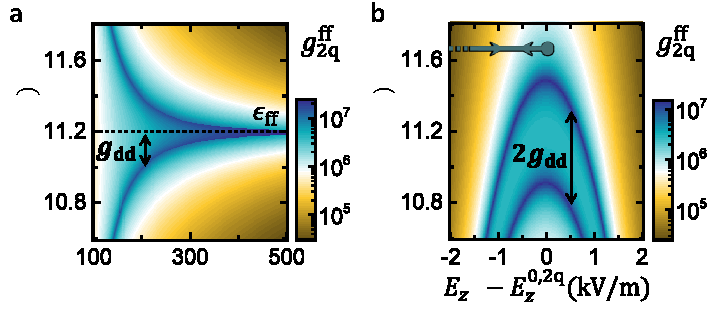
\includegraphics[width=\columnwidth]{polished/2qubit.pdf}
	\caption[Coupling rate between 2 flip-flop qubits]{\textbf{Coupling rate between 2 flip-flop qubits. a}, Effective coupling between 2 flip-flop qubits as a function of $V_{t,1}=V_{t,2}=V_t$, interdistance $r$ (\textbf{a}) and electric field $E_{z,1}=E_{z,2}=E_z$ (\textbf{b}). The arrows in \textbf{b} represent the adiabatic path followed for 2-qubit gates. $E_z^{\rm 0,2q}$ is the ionization point in the presence of a second qubit, $E_z^{\rm 0,2q}=E_z^0-2g_{\rm dd}h/(2eL_i)$.}
	\label{fig:2-qubit}
\end{figure}

The coupling rate exceeds $10$~MHz around two narrow regions when the flip flop qubit is in resonance with a molecular state as the two charge qubits in Fig.~\ref{fig:dipole}b form hybridized molecular states, which are coupled to each flip-flop qubit as illustrated in figure \ref{fig:dipole}c. The states of the hybridized molecular states are
 
\begin{eqnarray}
\tilde{g}=\beta\ket{eg}+\alpha\ket{ge}\\
\tilde{e}=-\alpha\ket{eg}+\beta\ket{ge}
\end{eqnarray}

,similar to eq. \eqref{eq:hybridstates}, with the coefficients as in eq. \eqref{eq:ab} and\eqref{eq:abcont}. We have $A=\delta_{so,2}-\delta_{so,1}$ and $B=2g_{dd}$. Basically A describes the energy scale ($\sigma_z$) and B drives the transitions ($\sigma_x$). 
The coupling between the two charge qubits shifts the charge qubit eigenenergies.

The resonant regime, however, induces too many relaxation errors due to resonant charge excitation. Therefore it is best to detune the flip-flop qubits from the molecular states, while still keeping a substantial inter-qubit coupling rate, via a second-order process.
 We calculate this coupling rate between the flip-flop qubits to 
 
 \begin{eqnarray}\label{eq:flipdipSWAP_Delta}
g_{\rm 2q}^{\rm ff} &=& \bra{\uparrow_1\Downarrow_1 \downarrow_2\Uparrow_2 \tilde{g}}H_{tot}\ket{\downarrow_1\Uparrow_1 \uparrow_2\Downarrow_2 \tilde{g}} \\
& =& g_{\rm so,1}g_{\rm so,2}\alpha\beta\left(\frac{1}{D_{\rm dd}-\delta_{\rm so,1}}+\frac{1}{D_{\rm dd}+\delta_{\rm so,2}}\right)
\end{eqnarray}
where 

\begin{eqnarray}\label{eq:Ddd}
D_{\rm dd}&=&\frac{\left| \langle g_1 e_2|H_{orb}^A+H_{dip}\ket{e_1 g_2}\langle e_1 g_2 |H_{orb}^A +H_{dip}\ket{g_1 e_2 }\right|}{E_{e_1 g_2}-E_{g_1 e_2}}\\
& = & (\delta_{\rm so,2}-\delta_{\rm so,1})\left(1+[2g_{\rm dd}/(\delta_{\rm so,2}-\delta_{\rm so,1})]^2\right)/2
\end{eqnarray}

 is the charge eigenenergy shift.

Figure \ref{fig:2-qubit}b shows the coupling rate as a function of electric field at a fixed inter-qubit distance of $r=180\,$nm. 


\paragraph{Two-qubit gates}

2-qubit gates start with both electrons at the interface, where qubits are decoupled since the electric dipoles and the hyperfine interactions are first-order insensitive to vertical electric fields. Indeed, from Eq.~\ref{eq:flipdipSWAP_Delta}, $g_{\rm 2q}^{\rm ff}$ is negligible since $g_{\rm so}$ vanishes and $\delta_{\rm so}$ diverges. The electrons are then simultaneously and adiabatically displaced to the ionization point for a time necessary for an $\sqrt{i\mathrm{SWAP}}$ gate, before returning to the interface. 

\begin{figure}[h]
	\centering
	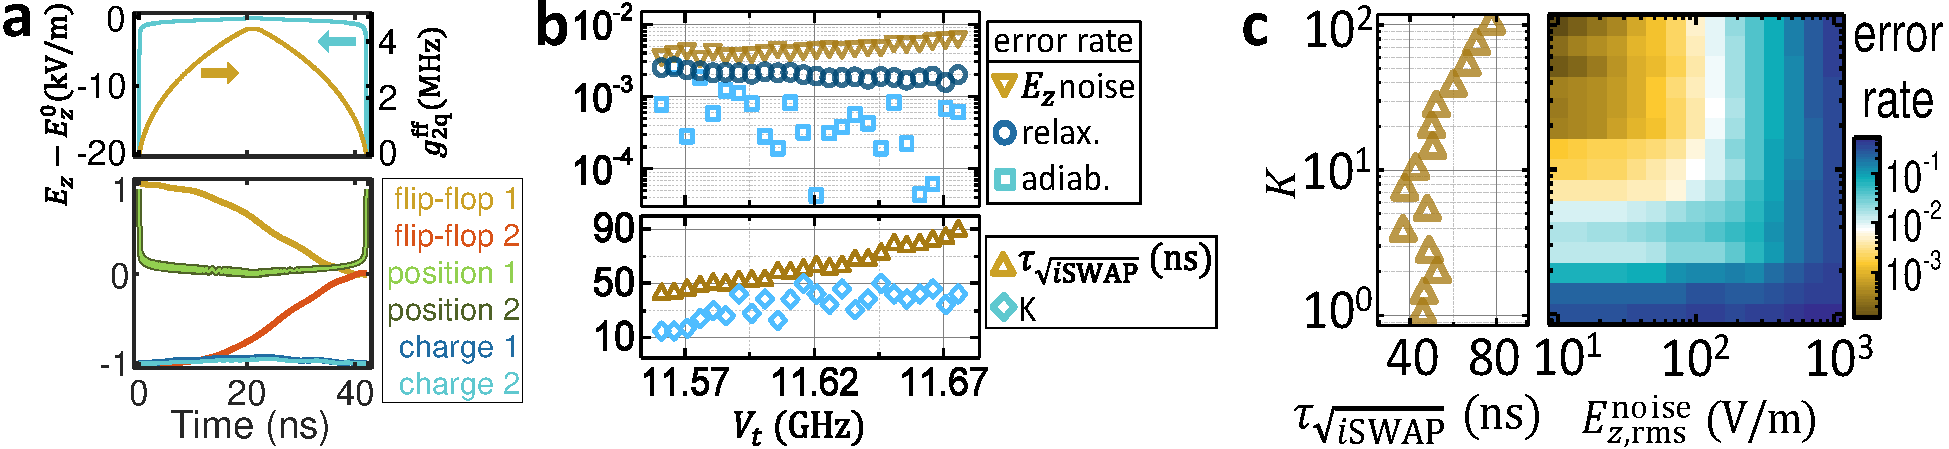
\includegraphics[width=1\columnwidth]{polished/iSWAP.pdf}
	\caption[High-fidelity adiabatic $\sqrt{i{\rm SWAP}}$ gates between two distant flip-flop qubits]{\textbf{High-fidelity adiabatic $\sqrt{i{\rm SWAP}}$ gates between two distant flip-flop qubits.}
		\textbf{a}, Time evolution of an adiabatic $\sqrt{i \rm SWAP}$ gate, for $K=30$, $r=180$~nm, $B_0=0.4$~T and $V_t=11.58$~GHz.
		\textbf{b}, Optimized $\sqrt{i{\rm SWAP}}$ gate error, gate time and adiabatic factor $K$.
		\textbf{c}, Optimized error rate arising from quasi-static $E_z$-noise, for different noise amplitudes and adiabatic factor $K$ (which sets the gate time).}
	\label{fig:iSWAP}
\end{figure}


In Fig.~\ref{fig:iSWAP}a we show the dynamics of a 2-qubit gate performed with an adiabatic factor $K=30$, following the trajectory shown in Fig.~\ref{fig:2-qubit}b. Similarly to 1-qubit $z$ gates (the calculations are analogous to those in adiabatic phase control), the electron is first displaced in a fast time scale ($\sim0.3$~ns) set by the charge qubit parameters ($\epsilon_{\rm o}$ and $V_t$), followed by a slower sweep ($\sim19$~ns) set by the spin-charge coupling parameters ($\delta_{\rm so}$ and $g_{\rm so}$), until it reaches the ionization point. The electron remains still for a short time before the whole process is then reversed. In the end a $\sqrt{i\mathrm{SWAP}}$ gate is performed. While some amount of charge is excited during the process, it goes back to its ground state, $\ket{gg}$, with an adiabatic error around $10^{-3}$.

We quantify the 2-qubit gate fidelity in presence of the most deleterious noise types for our qubits, namely quasi-static $E_z$ noise and charge-phonon relaxation. For this, we observe that the optimal gate fidelities are achieved when $E_z(\tau_{\sqrt{i\mathrm{SWAP}}}/2)\approx E_z^0$. Similarly to 1-qubit $x$-gates, this happens because $\sqrt{i\mathrm{SWAP}}$ gates are sensitive to gate time jitter, and therefore errors are minimized at the CQSS where $g_{\rm 2q}^{\rm ff}$ is robust against $E_z$ noise to first order -- recall Fig.~\ref{fig:2-qubit}e and Eq.~\ref{eq:flipdipSWAP_Delta}). An optimization algorithm finds the best adiabatic factor $K$ that minimizes errors due to $E_z$ noise for each value of $V_{t,1}=V_{t,2}=V_t$. The result is shown in Fig.~\ref{fig:iSWAP}b. Smaller detunings $\delta_{\rm so}$ (small $V_t$) result in shorter gate times, which in turn reduces errors from quasi-static noise. However, this also implies a larger admixture of charge in the qubit eigenstates, which slightly increases relaxation errors. The lowest error rates, $\sim3\times10^{-3}$ are found at small detunings, $V_t-\epsilon_{\rm ff}-g_{\rm dd}\approx 100$~MHz ($V_t\approx11.59$~GHz). At even smaller detunings, the 2-qubit coupling rate becomes too fast, requiring faster adiabatic sweeps to avoid over-rotation (lower $K$, Fig.~\ref{fig:iSWAP}b) and generating more leakage errors. The gate errors remain within $10^{-3}-10^{-2}$ for a wide range of $V_t$. Finally, we estimate in Fig.~\ref{fig:iSWAP}c how noise errors depend on the noise amplitude and adiabatic factor $K$, which sets the gate time.

Our proposed 2-qubit gates are not only well protected against noise, but also robust against donor misplacement. Variations in $r$, $d_1$ and $d_2$ mainly cause variations in the charge qubits coupling $g_{\rm dd}$, therefore simply changing the energy separation between molecular charge states (Fig.~\ref{fig:2-qubit}c). However, the coupling $g_{\rm 2q}^{\rm ff}$ between the flip-flop qubits can be kept essentially constant by simply readjusting $V_t$, using $e.g.$ the method described in Fig.~\ref{fig:clock}f,g. Figure~\ref{fig:2-qubit}d shows that one can keep a constant value of, for example, $g_{\rm 2q}^{\rm ff} = 1$~MHz for any inter-donor spacing between 180 and 500 nm, by adjusting $V_t$ between 11.3 and 11.8 GHz. In other words, since the flip-flop qubit coupling is mediated by a tunable interaction with their respective charge qubits, the inter-qubit interaction does not need to decay with $r^3$, as one would otherwise get when the dipole interaction couples the qubits directly \cite{Ogorman2014,Hill2015}. Therefore, two-qubit operations can be turned on between pairs of qubits separated by many sites in a 2-dimensional array. This tunable long-range connectivity can be exploited to great advantage in large-scale quantum processors \cite{Li2017}. The large tolerance in $g_{\rm dd}$ also accommodates very well the donor depth uncertainties inherent to ion implantation \cite{Donkelaar2015}, given the linear dependence of $g_{\rm 2q}^{\rm ff}$ on $d_i$ (Eqs. \ref{eq:V_dd} and \ref{eq:g_dd}).  

We conclude that our scheme provides a dramatic reduction in the fabrication complexity, especially compared to schemes that require placing a gate between a pair of tightly-spaced donors, such as the Kane's proposal \cite{Kane1998}, which requires $r\approx15$~nm separation between two $^{31}$P nuclear spins. Note that, by relocating the problem of valley oscillations from the exchange interaction \cite{Kane1998} to the tunnel coupling, we have effectively provided a way in which the delicate parameter can now be tuned using a much simpler gate geometry.


\section{Scaling up using circuit quantum electrodynamics}

\begin{figure}
	\centering
	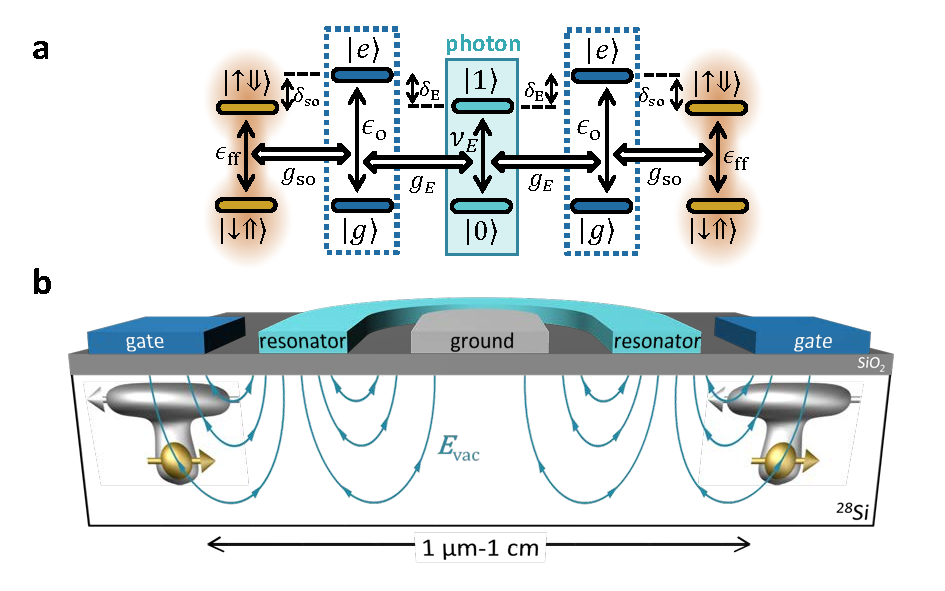
\includegraphics[width=\textwidth]{polished/cqed.pdf}
	\caption[Coupling to a resonator]{\textbf{Coupling to a resonator}.
		\textbf{a}, Level diagram for distant flip-flop qubit coupling via a microwave resonator showing photon number states and off-resonant charge states. 
		\textbf{b}, Device scheme for coupling qubits via a photonic link. Distant donors, placed next to the resonator center line and biased to their ionization point, are subject to the vacuum electric field $\textit{\textbf{E}}_{\rm vac}$ of a shared microwave resonator.}
	\label{fig:cqed}
\end{figure}

In order to reach the long-term goal of a large-scale quantum processor, wiring up the control and read-out lines for each individual qubit is not trivial, given the high density in typical spin qubit architectures \cite{Vandersypen2016}. Recent solutions include cross-wiring using multilayer lithography \cite{Hill2015} or floating gate electrodes inspired by dynamic random access memory systems \cite{Veldhorst2016}. In both cases, using flip-flop qubits with long-distance interactions would result in widely spaced donors and loose fabrication tolerances. In addition, since flip-flop qubits are coupled via electric fields, they could be spaced further apart by using electrical mediators. These include floating metal gates \cite{Trifunovic2012} or even microwave resonators. Indeed, the use of electric dipole transitions allows a natural integration of donor-based spin qubits into a circuit-Quantum Electrodynamics (QED) architecture \cite{Blais2004,Childress2004,Xiang2013,Mi2016} (see Fig. \ref{fig:processor}c for a possible device layout).

A full quantum mechanical treatment yields a charge-photon coupling rate given by Eq. \ref{eq:g_E}, with $\nu_E$ now representing the resonator fundamental mode frequency and $E_{\rm ac}$ the resonator vacuum field, $E_{\rm vac}$ . Again, it is best to have the charge excited state detuned from the flip-flop transition and resonator photon (see Fig. \ref{fig:processor}b), therefore minimizing charge excitation while retaining a second-order flip-flop-photon coupling given by Eq. \ref{eq:g_E_ff}. Assuming $\delta_{\rm so}\approx\delta_E\approx 10g_{\rm so}\approx 10g_E$, a $d=15$~nm deep $^{31}$P flip-flop qubit would be coupled to photons at a $g^{\rm ff}_E\approx3$~MHz rate. This is three orders of magnitude faster than the electron-spin coupling rate to a resonator via its magnetic vacuum field \cite{Tosi2014,Haikka2017}, and comparable to the coupling strength obtained by using strong magnetic field gradients \cite{Hu2012,Viennot2015}, but without the need to integrate magnetic materials within a superconducting circuit. This assumes a vacuum field amplitude $E_{\rm vac}\approx 30$~V/m, which can be obtained by using tapered coplanar waveguide or high-inductance resonators \cite{Samkharadze2016}.

The possibility of coupling the qubits to microwave photons provides a path for dispersive qubit readout, as well as for photonic interconnects. Near-quantum limited amplifiers have recently become available to obtain excellent readout speed and fidelities \cite{Castellanos2008}. The resonator can also be used as a quantum bus to couple two spin qubits separated by as far as 1~cm (Fig. \ref{fig:processor}c), a distance given by the mode wavelength. Fig. \ref{fig:processor}b shows the detailed energy level diagram. To avoid losses from photon decay, the qubits should be detuned from the resonator by an amount much greater than the qubit-photon coupling rates. Assuming $\delta^{\rm ff}_E=10g_{E}^{\rm ff}$, where $\delta^{\rm ff}_E=\nu_E-\epsilon_{\rm ff}$, the effective 2-qubit coupling $g_{\rm 2q}^{\rm ff}\approx(g_E^{\rm ff})^2/\delta^{\rm ff}_E\approx 0.3$~MHz yields a $\sqrt{i\mathrm{SWAP}}$ gate that takes only $0.4~\mu$s.


\begin{figure}
	\centering
	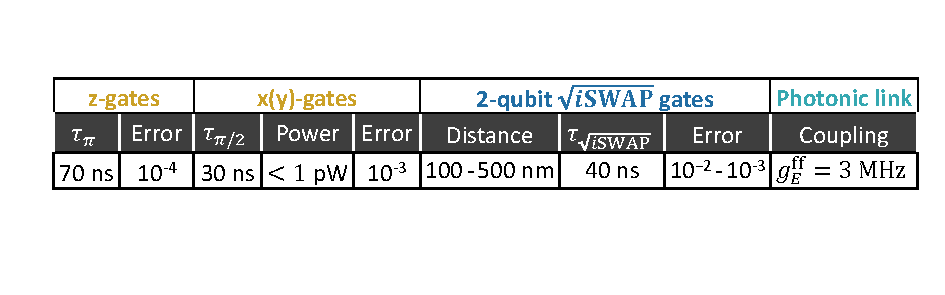
\includegraphics[width=\textwidth]{polished/merits.pdf}
	\caption[Gate performance summary summary]{\textbf{Gate performance summary}. Figures of merit summarizing the speed and error rates of different gate schemes present in this chapter, assuming realistic noise sources. }
	\label{fig:performance}
\end{figure}